\documentclass[12pt, letterpaper]{article}
\usepackage{graphicx} % Required for inserting images
\usepackage{hyperref}

\usepackage{amssymb}
\usepackage{amsmath}
\usepackage[english]{babel}
\usepackage{nicefrac, xfrac}
\usepackage{epsfig}
\usepackage[table,xcdraw]{xcolor}
\newcommand{\Z}{{\mathbb Z}}
\newcommand{\R}{{\mathbb R}}
\newcommand{\N}{{\mathbb N}}
\newcommand{\E}{{\mathbb E}}
\newcommand{\V}{{\mathbb V}}
\newcommand{\acc}{\\\hphantom{}\\}
\newcommand{\Prob}{{\mathbb P}}
\newcommand{\spaz}{{\text{\hphantom{aa}}}}
\newcommand{\pspace}{\((\Omega,\Prob)\)}
\usepackage[paper=a4paper,left=20mm,right=20mm,bottom=25mm,top=25mm]{geometry}
\title{Calcolo delle Probabilità}
\author{Marco Casu}
\date{\vspace{-5ex}}
\begin{document}



\maketitle
\begin{figure}[h]
    \centering{
    
\includegraphics[width=0.9\textwidth ]{images/cop.jpeg}
    }
\end{figure}
\newpage
\tableofcontents
\newpage
\section{Il Modello Probabilistico}
\subsection{Il Problema dei Compleanni}
Quante sono le probabilità che in un gruppo di 25 persone, 2 di queste siano nate lo stesso giorno? 
Procediamo nel \textbf{modellizzare} tale problema.
Le possibili date di nascita sono 365. 
\centering\(PossibiliDate=\{1,2,3,4...,365\}\)\\
\raggedright Intervistando un singolo individuo, questo può darmi 365 risposte, la probabilità che quindi
un individuo di nome \textit{Tizio} sia nato lo specifico giorno \(i\) è di 1 su 365.\\
\centering\( \mathbb{P}(\text{\textit{Tizio} è nato il giorno } i) = \dfrac{1}{365} \)\\
\raggedright Tale probabilità si dice \textbf{uniforme} perchè tutti i 365 esiti hanno la stessa
probabilità di \(\frac{1}{365}\) di risultare.
Adesso, quante sono le probabilità che \textit{Tizio} sia nato il giorno \(i\) e \textit{Caio}
il giorno \(j\)?\\
\centering\( \mathbb{P}(\text{\textit{Tizio} è nato } i \text{ e \textit{Caio} è nato } j) = \mathbb{P}(\text{\textit{Tizio} è nato il giorno } i) \cdot \mathbb{P}(\text{\textit{Caio} è nato il giorno } j) \)\\
\raggedright Questo si chiama \textbf{concetto di indipendenza}, ed è ovvio che le probabilità sono precisamente \(\dfrac{1}{365}\cdot\dfrac{1}{365} = \bigg( \dfrac{1}{365}\bigg)^2 \).
Quindi le probabilità che 25 persone siano nate in 25 giorni pre determinati sono precisamente : \\
\centering\( \mathbb{P}( a_1 \text{ è nato } i_1,a_2 \text{ è nato } i_2...,a_{25} \text{ è nato } i_{25}) = \bigg( \dfrac{1}{365}\bigg)^{25} \)\\
\raggedright
Queste sono le probabilità che 25 persone siano nate lo stesso giorno, a noi ci interessano però
le probabilità che almeno 2 persone siano nate lo stesso giorno. Prima di fare ciò andiamo a definire
quello che si dice \textbf{modello probabilistico}.\\
Chiamiamo \(\Omega\) lo spazio degli eventi elementari (in seguito verrà definito in modo formale), 
Ossia l'insieme di tutti i possibili risultati dell'esperimento. Sia l'esperimento in questo caso, la 
data di nascita per \(k\) persone, il nostro \(\Omega\)  sarà l'insieme di tutte le possibili combinazioni 
lunghe 25 di  numeri da 1 a 365, che sono precisamente \(|\Omega|=365^{25}\). La probabilità uniforme
che un certo evento dello spazio degli eventi \(\Omega={\omega_1,\omega_2...,\omega_k }\) accada è \(\mathbb{P}({\omega_i})=\dfrac{1}{|\Omega|}\).
Definiamo adesso un evento \textbf{binario}, ossia un evento che ha come risposta, o si o no,ossia le probabilità che 
esso accada e che esso non accada. Definiamo l'evento \(A\) come l'evento in cui almeno 2 persone fanno il compleanno
lo stesso giorno.\\
\centering\( A=\{\omega \in \Omega :\exists \omega_i,\omega_j \in \omega | i\ne j \land \omega_i=\omega_j\} \)\\
\raggedright
Quindi tale \(A\) è un sottoinsieme di \(\Omega\) in cui tutti gli elementi hanno almeno 2 date uguali. 
Presa con \(|A|\) la cardinalità di tale sottoinsieme, le probabilità che tale evento accada sono :\\
\centering\( \mathbb{P}(A)=\dfrac{|A|}{|\Omega|} \)\\
\raggedright Piuttosto che trovare l'evento in cui ci sono almeno 2 persone con lo stesso  compleanno,
è più facile trovare il suo \textbf{complementare}, ossia l'evento in cui nessuno fa il compleanno lo stesso giorno.
\\\centering\( A^c=\{\omega \in \Omega | \forall i\ne j, \omega_i \ne \omega_j\} \)\\
\raggedright Una volta trovata la probabilità di \(A^c\), sapremo che \(\mathbb{P}(A)=1-\mathbb{P}(A^c)\).
\\\centering essendo \(k=25 \) e \( n=365 \rightarrow |A^c|=n \cdot (n-1) \cdot (n-2)...\cdot (n-k+1)  \implies
 \mathbb{P} (A)=1-\dfrac{|A^c|}{365^{25}}\)  \\
\raggedright Vediamo una tabella di possibili risultati al variare di \(k\) (numero di persone) :\\\hphantom{.}\\
\centering
    \begin{tabular}{|l|l|l|l|l|l|}
    \hline
    \(k\)  & 4    & 16   & 22   & 23   & 63   \\ \hline
    \(\mathbb{P}(A)\) & 0.06 & 0.28 & 0.42 & 0.50 & 0.99 \\ \hline
    \end{tabular}
\\\raggedright
 Risulta chiaro come, intervistando 25 persone, c'è una probabilità superiore 
al 50 \% che almeno due di esse condividano il compleanno.
\subsection{Assiomi della probabilità}
Definiamo adesso formalmente il \textbf{modello probabilistico}, esso ha 3 ingredienti :
\\\hphantom{.}\\\textbf{1 - Lo Spazio degli Eventi Elementari}

Detto anche \textit{spazio campionario}, non è altro che l'insieme di tutti i possibili esiti dell'
esperimento, e viene denominato con \(\Omega\). Ad esempio, se l'esperimento è il lancio di una moneta,
si avrà \(\Omega=\{\)Testa,Croce\(\}\). Nel caso dell'esperimento dei compleanni, lo spazio campionario 
sarà composto da tutte le possibili combinazioni lunghe \(k\) ( numero di persone alla quale si chiede 
la data di nascita ) di numeri da 1 a 365 (i giorni esistenti). Per la maggior parte dei casi analizzati 
in questo corso, \(\Omega\) sarà un insieme finito. Si indica con \(|\Omega|\) la cardinalità dello 
spazio campionario, ossia il numero dei suoi elementi.
\\\hphantom{.}\\\textbf{2 - Algebra degli Eventi}

Prima di definire l'algebra degli eventi, dichiariamo cos'è un \textbf{evento}, ossia una \textit{domanda
binaria} sull'esito dell'esperimento, in termini matematici, è un qualsiasi sottoinsieme \(\Omega\), compresi
gli elementi singoli di \(\Omega\), detti \textbf{eventi elementari}. Se l'esperimento è il lancio di un dado,
i possibili esiti sono \(\Omega=\{1,2,3,4,5,6\}\), vogliamo definire l'evento \(A\) come la probabilità
che l'esito del lancio sia un numero maggiore di 4, esso non è altro che un sottoinsieme dello spazio campionario,
ossia \(A=\{\omega \in \Omega | \omega \ge 4 \}=\{4,5,6\}\). 

Su tali eventi sono definite delle operazioni insiemistiche di unione, intersezione e complemento.\\
L'Algebra degli Eventi, definita con il simbolo \(\mathcal{A} \), è l'insieme chiuso\footnote{
    È un insieme chiuso rispetto alle operazioni di unione, intersezione e complemento, ossia il risultato
    di tali operazioni su uno o più elementi dell'insieme, è sempre parte di tale insieme.
    } 
 di \textit{tutti
i possibili sotto-insiemi} dello spazio campionario, ossia tutti i possibili eventi 
(anche non elementari) per la quale si può misurare la probabilità. 
\textit{Ad esempio}, se prendiamo il caso del dado \(\Omega=\{1,2,3,4,5,6\}\), l'evento
in cui il risultato sia 2 o 3, è l'unione dei due eventi elementari \(A=\{2\}\) e \( B=\{3\} \rightarrow C = A \cup B
= \{2,3\}\). Si noti che \(|\Omega|=n \implies |\mathcal{A}|=2^n\)
\\\hphantom{.}\\\textbf{3 - La Funzione Probabilità}
La probabilità di un determinato evento appartenente ad \(\mathcal{A} \) è misurata tramite una 
funzione definita come \(\mathbb{P} : \mathcal{A} \rightarrow [0,1]\), essa associa ad ogni elemento
dell'algebra degli eventi, una probabilità misurata tra 0 ed 1, dove 0 indica che l'evento è impossibile,
ed 1 che l'evento è certo. La funzione \(\mathbb{P}\) deve soddisfare 3 condizioni :
\begin{itemize}
    \item \(\mathbb{P}(\emptyset )= 0\) La probabilità dell'insieme vuoto è 0.
    \item \(\mathbb{P}(\Omega)= 1\) La probabilità che si verifichi un evento di \(\Omega\) è l'evento certo.
    \item \(\mathbb{P}\) è una funzione \textit{additiva}, ossia che per due eventi disgiunti \(A\) e 
    \(B\), nel senso che \(A\cap B = \emptyset\), vale che \(\mathbb{P}(A\cup B)=\mathbb{P}(A)+\mathbb{P}(B)\).
\end{itemize}
Vediamo adesso \textbf{alcune considerazioni} riguardo gli assiomi appena enunciati.\\
Risulta ovvio che \(\Omega = A\cup A^c \implies \mathbb{P}(A^c)=1-\mathbb{P}(A)\). Diversamente, presi 
due eventi \(A\) e \(B\) \textit{non necessariamente disgiunti}, vale che \(\mathbb{P}(A\cup B)
=\mathbb{P}(A)+\mathbb{P}(B)-\mathbb{P}(A\cap B)\). Un'altra considerazione, è che \(\mathbb{P}\)
 è una funzione \textit{monotona} rispetto all'inclusione di insiemi, detto formalmente 
 \(A \subseteq B \implies \mathbb{P}(A) \le \mathbb{P}(B)\).
\\ Quando si vuole misurare la probabilità di un evento in un certo 
esperimento, bisogna quindi costruire un modello probabilistico, definendone gli eventi elementari e
 la probabilità ad essi associati. Possiamo quindi definire un altra funzione \(p\), che ha come dominio
 esclusivamente gli eventi elementari \(\Omega\), e non gli eventi di \(\mathcal{A}\), essa sarà 
 denominata come \textbf{probabilità degli eventi elementari}, \(p:\Omega \rightarrow [0,1]\). Risulta
 chiaro che \(\displaystyle\sum_{\omega \in \Omega} p(\omega)=1  \).\\
 Ad esempio, facciamo un esperimento sul lancio di un dado truccato in cui è più probabile che esca 
 il numero 6 piuttosto che altri :
 \\ \center \(\Omega=\{1,2,3,4,5,6\}\)\\
 \raggedright\( p(1)=p(2)=p(3)=0.1\)\\\( p(4)=p(5)=0.2\)\\\(p(6)=0.3\)
 \\
 Definiamo quindi \(\displaystyle\mathbb{P}(A)=\sum_{\omega \in A}p(\omega)\), e risulta chiaro che :\\
 \centering
 \(\displaystyle\sum_{\omega \in \Omega}p(\omega)=\sum_{\omega \in A}\mathbb{P} (\{\omega\})=
 \mathbb{P}(\bigcup_{\omega \in \Omega}\{\omega\} )=1\)
 \\\raggedright La probabilità in un modello probabilistico, si dice \textbf{uniforme} se \(p(w)=\dfrac{1}{|\Omega|} \) \(\forall \omega \in \Omega\)
, e significa che tutti gli eventi elementari hanno la stessa probabilità di accadere, da qui ne deriva che la 
probabilità di un evento \(A\in \mathcal{A} \) è \(\mathbb{P}(A)=\dfrac{|A|}{|\Omega|}\).
\section{Calcolo Combinatorio}
Riassumiamo in questa sezione ciò che si è visto nel corso di \textit{Metodi matematici per l'informatica}. Partiamo
con un problema, si dia il caso che in un urna ci sono 3 palline bianche e 2 palline nere, qual'è la probabilità che, 
estraendo due palline, la seconda sia bianca? Formalizziamo il problema secondo il modello probabilistico.
L'evento elementare è l'estrazione \textit{ordinata} di due palline \(\omega=(\omega_1,\omega_2)\), dove 
\(\omega_1\) = prima estratta e \(\omega_2\) = seconda estratta. Possiamo numerare le palline da 1 a 5, 
dicendo che le palline bianche son quelle da 1 a 3, e le restanti le nere. Detto ciò, possiamo capire che l'insieme 
degli eventi elementari, sono tutte le coppie di numeri naturali compresi fra 1 a 5 senza ripetizioni.
\begin{equation}
    \Omega = \{(w_1,w_2) | w_1,w_2 \in \{1,2,3,4,5\}, w_1 \ne w_2\}
\end{equation}
È di facile intuizione capire che \(|\Omega|=20\).\\
L'evento \(A\) invece rappresenta il sottoinsieme di \(\Omega\), dove 1,2 o 3 appaiano sempre come seconda 
coordinata dei suoi elementi, ossia tutte le estrazioni in cui la seconda pallina è bianca. Per calcolare \(\mathbb{P}(A)\),
dobbiamo capire qual'è prima la cardinalità di \(A\), che risulta essere \(|A|=3\cdot 4 = 12\), il 3 rappresenta 
le 3 possibili palline bianche della seconda estrazione, il 4 invece tutte le altre possibili rimanenti (per
 la quale non ci interessa il colore essendo la prima estrazione.) Fatto ciò si ha \(\mathbb{P}(A)=\dfrac{|A|}{|\Omega|}=\dfrac{12}{20}=\dfrac{3}{5}=0.6\). La 
 probabilità è quindi del 60\%.
 \subsection{Principio fondamentale del calcolo combinatorio}
 Dati due insiemi finiti e non vuoti \(A\) e \(B\), è possibile formare \(|A|\cdot|B|\) diverse coppie ordinate 
 prendendo un primo elemento da \(A\) ed un secondo elemento \(B\).
 \begin{equation}
    |A\times B|=|A|\cdot|B|
 \end{equation}
 \newpage Vediamo un \textit{esempio} :\\
 Lanciamo un dado 6 volte, quant'è la probabilità che esca almeno una delle volte 6? Diciamo che un evento 
 elementare \(\omega\) è una ennupla di 6 elementi (i lanci) composta da numeri da 1 a 6 (esiti del dado). 
 \begin{equation}
    \Omega = \{(\omega_1,\omega_2,...\omega_6) | \omega_i \in \{1,2,3,4,5,6\}\}
 \end{equation}
 Risulta chiaro (per il principio moltiplicativo) che \(|\Omega|=6^6\).
 Dobbiamo adesso calcolare la cardinalità di \(A=\{\omega \in \Omega | \exists \omega_i \in \omega \rightarrow\omega_i = 6\}\),
 ossia tutti gli eventi elementari in cui 6 compare almeno in un lancio. Ci risulta però più facile calcolare il 
 suo complementare, ossia tutti gli eventi in cui 6 non compare mai, ossia
 ogni ennupla di 6 elementi (i lanci) composta da numeri da 1 a 5 (esiti del dado escluso il 6). 
 \begin{equation}
    A^c = \{(\omega_1,\omega_2,...\omega_6) | \omega_i \in \{1,2,3,4,5\}\}
 \end{equation}
 Risulta chiaro (per il principio moltiplicativo) che \(|A^c|=5^6\).
 Avendo la \(|A^c|\), possiamo trovare la probabilità dell'evento \(A\) : 
 \begin{equation}
    \mathbb{P}(A)=1-\mathbb{P}(A^c)=1-\dfrac{|A^c|}{|\Omega|}=1-\dfrac{5^6}{6^6}\simeq 0.66
 \end{equation}
 \subsection{Modelli del calcolo combinatorio}
 Prima di parlare dei modelli del calcolo combinatorio, introduciamo un concetto importante :
 \begin{quote}
    \textbf{Permutazione}\\
    Sia \(S\) un insieme finito e non vuoto, una \textit{permutazione} di \(S\) è 
    una scelta di ordine tra gli elementi di \(S\). Le possibili permutazioni risultano essere \(|S|!\) .
 \end{quote}
 Passiamo adesso alla presentazione di alcuni modelli fondamentali nella quale spesso ricadono i problemi 
 di conteggio. I problemi verranno \textit{metaforizzati} secondo il problema delle palline nelle urne.
 \subsubsection{Caso 1 - Estrazioni Ordinate con Rimpiazzo}
Si hanno \(n\) palline dentro un urna e si vogliono fare \(k\) estrazioni con rimpiazzo, ossia, una volta
pescata una pallina, si reinserisce nell'urna (un elemento stesso può essere estratto più volte). Si tiene 
conto dell'ordine, quindi \(\{1,2,3\}\ne\{1,3,2\}\). Per problemi di questo tipo, vale che : 
\begin{equation}
    \Omega = \{(\omega_1,\omega_2...,\omega_k) | \omega_i \in \{1,2,3...,n\}\} \implies |\Omega|= n^k
\end{equation}
\subsubsection{Caso 2 - Estrazioni Ordinate senza Rimpiazzo}
Si hanno \(n\) palline dentro un urna e si vogliono fare \(k\) estrazioni senza rimpiazzo, ossia, una volta
pescata una pallina, essa non potrà essere ripescata (gli elementi di ogni estrazione sono distinti). Si tiene 
conto dell'ordine, quindi \(\{1,2,3\}\ne\{1,3,2\}\). Per problemi di questo tipo, vale che : 
\begin{equation}
    \Omega = \{(\omega_1,\omega_2...,\omega_k) | \omega_i \in \{1,2,3...,n\}|i\ne j \implies w_i\ne w_j\} \implies |\Omega|= \dfrac{n!}{(n-k)!}
\end{equation}
\textit{Esempio :}\\
7 persone si trovano in un ascensore dentro un palazzo di 10 piani e si apprestano a scendere su un piano,
quante sono le probabilità per cui tutte quante scendano su piani diversi? L'Evento elementare è 
composta da una ennupla di 7 elementi (le persone) composta da numeri che vanno da 1 a 10 (il piano in cui scendono).
Quindi : \\\begin{center} \(\Omega = \{(\omega_1,\omega_2...,\omega_7)|\omega_i = \{1,2,3,4,5,6,7,8,9,10\}\}\)
\end{center}
Dati i modelli precedenti risulta chiaro che \(|\Omega|=10^7\) e \(A=\{\)Ognuno scende su un piano diverso\(\}\) ha cardinalità
 \(|A|=\dfrac{10!}{3!}\implies \mathbb{P}(A)=\dfrac{\frac{10!}{3!}}{10^7}\simeq0.06\) .
 \subsubsection{Caso 3 - Estrazioni non Ordinate senza Rimpiazzo}
 Si hanno \(n\) palline dentro un urna, se ne estraggono \(k\), ma senza tener conto dell'ordine delle palline, ad esempio,
 se ho le palline denominate 1,2 e 3, estraendole, si ha che le estrazioni 123, 321 ,132, 312, 231, 213 sono 
 lo stesso evento. Come rappresento tale spazio elementare \(\Omega\) a livello insiemistico? Si consideri lo spazio 
 delle \textit{Estrazioni Ordinate senza Rimpiazzo}, ossia:\begin{center} \( A  =\{(\omega_1,\omega_2...,
    \omega_k) | \omega_i \in \{1,2,3...,n\}|i\ne j \implies w_i\ne w_j\}\) \end{center}
Stabiliamo una relazione di equivalenza su \(A\), denominata con il simbolo \(\sim \), per cui 
vale che \(\omega\sim \omega'\) se e solo se differiscono solo per l'ordine. \\\textit{Esempio :}
\(\omega=\{1,2,3\},\omega'=\{3,1,2\}\iff \omega\sim \omega'\).
L'insieme degli eventi elementari per rappresentare le \textit{Estrazioni non Ordinate senza Rimpiazzo}
non è altro che l'insieme quoziente di \(A\) su \(\sim\), ossia l'insieme di tutte le sue classi di 
equivalenza.\begin{center}
    \(\displaystyle\Omega=\displaystyle\sfrac A\sim\)
\end{center}
Possiamo scegliere come rappresentanti delle classi di equivalenza, quegli elementi in cui le palline 
sono ordinate in ordine crescente, in tal modo, lo spazio elementare è anche rappresentabile come :
\begin{center}
    \(
        \{(\omega_1,\omega_2...,\omega_k)|\omega_i \in \{1,2,3...,n\} \land i<j\implies w_i < w_j\}
    \)
\end{center}
Qual'è però la cardinalità di \(\Omega\) in questo caso? Possiamo considerare la cardinalità di \(A\), divisa 
per il numero di elementi in ogni classe di equivalenza. Essendo che ogni classe di equivalenza non è altro
permutazione di \(k\) elementi, esse avranno ognuna \(k!\) elementi, da qui risulta chiara la cardinalità del 
nostro spazio degli eventi :
\begin{equation}
    \text{sia } [\omega]\in \sfrac{A}{\sim} \text{,  si ha  } |\Omega|=\dfrac{|A|}{|[\omega]|}=\dfrac{n!}{k!\cdot(n-k)!} \text{ si denota come }\binom{n}{k} 
\end{equation}
Tradotto in linguaggio umano, \(\binom{n}{k}\) indica il numero di modi di scegliere \(k\) elementi da un insieme \(n\). Tale
conteggio è anche detto \textbf{combinazione semplice}.
Vale la proprietà : \begin{center}
    \(\displaystyle\binom{n+1}{k+1}=\binom{n}{k+1}+\binom{n}{k}\)
\end{center}
\large \textbf{Binomio di Newton}\\\begin{center}
\normalsize Siano \(a,b \in \mathbb{R}\) e \(n\in\mathbb{N}\), vale che \(
    \displaystyle(a+b)^n = \sum_{k=0}^{n}\binom{n}{k}\cdot a^{n-k}\cdot b^k
\)\end{center}
\subsubsection{Caso 4 - Estrazioni non Ordinate con Rimpiazzo}
\normalsize Consideriamo il lancio di 2 dadi identici, senza considerare l'ordine. Abbiamo che l'evento elementare 
è la coppia di numeri da 1 a 6 (senza contare l'ordine, quindi consideriamo la classe di equivalenza 
in cui i due dadi hanno esito in ordine crescente), lo spazio risulta quindi : \(\Omega=\{(\omega_1,\omega_2)|1\le\omega_1\le\omega_2\le 6\}\)
\\Se i due dadi fossero distinti e l'ordine avesse importanza, i possibili eventi sarebbero \(6^2\), ma in questo caso, 
non risulta la scelta naturale, dato che gli eventi \((a,b)\) e \((b,a)\) sono identici.\\\hphantom{.}\\ È il caso di un \textit{estrazione
non ordinata con rimpiazzo}, dato che estraggo due palline, senza contare l'ordine, con la possibilità di poter 
estrarre due volte la stessa pallina.\\
Se ho \(n\) palline e faccio \(k\) estrazioni, il numero di estrazioni possibili non ordinate con rimpiazzo 
risulta essere : \begin{equation}
    \binom{n+k-1}{k}
\end{equation}
Tornando al problema dei dadi, i possibili esiti sono : \begin{center}
    \(
        \displaystyle\binom{6+2-1}{2}=\dfrac{(6+2-1)!}{2!(6+2-1-2)!}=\dfrac{7!}{2!5!}=\dfrac{7\cdot6\cdot5\cdot4\cdot3\cdot2}{5\cdot4\cdot3\cdot2\cdot2}=\dfrac{7\cdot6}{2}=21
    \)
\end{center}
\subsection{Principio di Esclusione/Inclusione}
Siano \(A,B,C\subset \Omega\) tre eventi non necessariamente disgiunti di uno spazio di probabilità, se volessi 
calcolare la probabilità di \(A\cup B\), dovrei fare la somma delle probabilità di \(A\) e \(B\), sottraendo la 
probabilità dell'intersezione. Già con 3 eventi, se volessi la probabilità dovrei fare :
\begin{center}
    \(\mathbb{P}(A\cup B\cup C)=\mathbb{P}(A)+\mathbb{P}(B)+\mathbb{P}(C)-(\mathbb{P}(A\cap B)+\mathbb{P}(A\cap C)+\mathbb{P}(B\cap C))+\mathbb{P}(A\cap B \cap C)\)
\end{center}
Quando si parla quindi di un numero elevato di eventi, il calcolo risulta difficile, ed è descritto dalla seguente formula :
\begin{equation}
    \mathbb{P}(A_1\cup A_2...,\cup A_n)=\sum_{k=1}^n(-1)^{k+1}\cdot\sum_{1<i_1<i_2...,<i_k<n}\mathbb{P}(A_{i_1}\cap A_{i_2}...,\cap A_{i_k})
\end{equation}
\subsection{Il Multinomio}
Esaminiamo il problema in cui si vogliono distribuire \(n\) oggetti distinti in \(k\) scatole distinte, in modo che 
ciascuna di esse contenga nell'ordine \(n_1,n_2...,n_k\) oggetti, per cui \(\displaystyle\sum_{i=1}^n n_i =n\). In quanti modi posso 
effettuare tale suddivisione? Ci sono \(\binom{n}{n_1}\) scelte per la prima scatola, \(\binom{n-n_1}{n_2}\) per la seconda 
e così via, fino a \(\dfrac{n!}{n_1!\cdot n_2!...,\cdot n_k!}\), che si denota con \(\displaystyle\binom{n}{n_1,n_2...,n_k}\), e 
rappresenta il numero di suddivisioni di \(n\) oggetti distinti in \(k\) gruppi distinti con, rispettivamente
\(n_1,n_2...,n_k\) oggetti.\\
\hphantom{.}\\\textit{Esempio : }Vi sono 10 poliziotti, se 5 di essi devono pattugliare due strade, 2 di essi 
restare in stazione ed altri 3 stare in riserva, quanti sono i modi possibili di assegnare i 3 compiti ai 
10 poliziotti? \begin{center}
    \(
      \displaystyle\binom{10}{5,2,3}=\dfrac{10!}{5!\cdot2!\cdot3!}=\dfrac{10\cdot9\cdot8\cdot7\cdot6\cdot5\cdot4\cdot3\cdot2}{5\cdot4\cdot3\cdot2\cdot 3 \cdot 2 \cdot 2}=\dfrac{30240}{12}=2520  
    \)
\end{center}
\subsection{Problema degli Accoppiamenti}
Poniamo un esempio, c'è una festa con \(n\) invitati, ogni invitato porta con se un ombrello, 
al termine della festa ogni invitato se ne va prendendo un ombrello a caso, qual'è la probabilità 
che nessun invitato riprenda il proprio ombrello? Se il numero di persone \(n\) tende ad 
infinito, come si comporta tale probabilità?\\\hphantom{.}\\ In uno spazio di probabilità, 
se un evento elementare composto da una lista \(a_1,a_2...,a_n\) che possono assumere 
valori da \(1\) ad \(n\), capita che un elemento \(a_i\) assume valore \(i\), esso si dice \textbf{punto fisso},
quindi possiamo tradurre il problema degli ombrelli (considerando ogni persona come un elemento dell'evento 
elementare, ed i valori che possono assumere come gli ombrelli) come : Qual'è la probabilità che una permutazione 
di \(n\) non abbia punti fissi?\begin{center}
    \(\Omega=\{(\omega_1,\omega_2...,\omega_n)|i\ne j \implies \omega_i\ne \omega_j |\omega_k \in \{1,2,3...,n\} \}\) dove \(|\Omega|=n!\)
    \\\(B=\{\)permutazioni senza punti fissi\(\}=\{\omega\in\Omega | \forall i \in\{1,2,3...,n\} \omega_i\ne i \}\)
\end{center}
Poniamo il complementare di \(B\), ossia \(B^c=A=\{\)la permutazione ha almeno un punto fisso\(\}\), e distinguiamolo 
in \(n\) sotto eventi, ossia \(A_1=\{\omega_1\) è un punto fisso\(\}\) poi 
\(A_2=\{\omega_2\) è un punto fisso\(\}\) e così via per ogni punto. Sapremo così che 
\(A=A_1\cup A_2..., \cup A_n\). Calcoliamo la cardinalità di un singolo evento \(A_i\), risulta 
facile, dato che poniamo un punto fisso su \(\omega_i = i\) e poi il resto è una permutazione 
normale. \(|A_i|=(n-1)!\), quindi \(\mathbb{P}(A_i)=\dfrac{(n-1)!}{n!}=\dfrac{1}{n}\). Quindi per calcolare 
la probabilità di \(A\) dobbiamo sommare le probabilità di ogni \(A_i\), ma ovviamente tali sotto-eventi 
\textit{non sono disgiunti}, quindi dobbiamo sottrarre le intersezioni.
Notiamo come \(|A_i\cap A_j|=(n-2)!\), perchè fissiamo entrambi i punti \(i,j\) e ed il resto 
è una semplice permutazione. Questo fino a \(k\) intersezioni : \(|A_1\cap A_2...,\cap A_k|=(n-k)!\). Quindi :
\(\mathbb{P}(A_1\cap A_2...,\cap A_k) =\dfrac{(n-k)!}{n!}\). A questo punto applichiamo qui il 
\textbf{principio di esclusione/inclusione} :\begin{equation}
    \mathbb{P}(\bigcup^n_{k=1}A_k )=\sum_{i=1}^n (-1)^{k+1}\sum_{1<i_1<i_2...,<i_k<n}\mathbb{P}(A_1\cap A_2...,\cap A_k)
\end{equation}
Ma sappiamo che \(\mathbb{P}(A_1\cap A_2...,\cap A_k) =\dfrac{(n-k)!}{n!}\) quindi riscriviamo :\begin{equation}
    \mathbb{P}(\bigcup^n_{k=1}A_k )=\sum_{i=1}^n (-1)^{k+1}\sum_{1<i_1<i_2...,<i_k<n}\dfrac{(n-k)!}{n!}
\end{equation}
\begin{equation}
    \mathbb{P}(\bigcup^n_{k=1}A_k )=\sum_{i=1}^n (-1)^{k+1}\binom{n}{k} \dfrac{(n-k)!}{n!}
\end{equation}
\begin{equation}
    \mathbb{P}(\bigcup^n_{k=1}A_k )=\sum_{i=1}^n (-1)^{k+1}\dfrac{n!}{(n-k)!k!} \dfrac{(n-k)!}{n!}
\end{equation}
\begin{equation}
    \mathbb{P}(\bigcup^n_{k=1}A_k )=\sum_{i=1}^n (-1)^{k+1}\dfrac{1}{k!}
\end{equation}
Essendo \(A\) il complementare di \(B\) :
\begin{equation}
    \mathbb{P}(B)=1-\sum_{i=1}^n (-1)^{k+1}\dfrac{1}{k!}
\end{equation}
Con \(n\) che tende ad infinito si ha :
\begin{equation}
    \lim_{n\rightarrow \infty }\mathbb{P}(B)=1-\sum_{i=1}^n (-1)^{k}\dfrac{1}{k!}=\dfrac{1}{e}
\end{equation}
Quindi la probabilità che in una permutazione non vi siano punti fissi è \textbf{costante}, e 
vale esattamente \(\dfrac{1}{e}\).
\section{Spazi di Probabilità Notevoli}
\subsection{Spazi di Probabilità Prodotto}
Consideriamo due esperimenti : \begin{itemize}
    \item Lancio una moneta equa 
    \item Viene misurata la temperatura in Brasile (che può variari dai 10 ai 50 gradi)
\end{itemize}
Per i due esperimenti diversi abbiamo due spazi di probabilità differenti, \((\Omega_1,\mathbb{P}_1)\) e 
\((\Omega_2,\mathbb{P}_2)\), considerando l'esperimento congiunto, essendo essi totalmente indipendenti (non si 
influenzano fra loro), possiamo immaginare ogni evento come una coppia composta dal primo evento elementare ed 
il secondo evento elementare, costruendo un nuovo spazio elementare come prodotto cartesiano
dei primi due : \(\Omega=\Omega_1\times\Omega_2\).\begin{center}
    \( \Omega=\{(\omega_1,\omega_2)|\omega_1\in\{T,C\}, \omega_2\in \mathbb{N} | 10\le\omega_2\le50 \)
\end{center}
Se i due esperimenti non si influenzano, la scelta naturale è la \textbf{probabilità prodotto} :
\begin{equation}
    \mathbb{P}(\{\omega\})=\mathbb{P}(\{(\omega_1,\omega_2)\})=\mathbb{P}_1(\{\omega_1\})\cdot\mathbb{P}_2(\{\omega_2\})
\end{equation}
Devo verificare che \(\displaystyle\sum_{\omega \in \Omega}\mathbb{P}(\{\omega\})=1\), ho che :
\begin{equation}
    \sum_{\omega \in \Omega}\mathbb{P}(\{\omega\})=\sum_{\omega \in \Omega}\mathbb{P}_1(\{\omega_1\})\cdot\mathbb{P}_2(\{\omega_2\})
\end{equation}
\begin{equation}
    \sum_{\omega_1 \in \Omega_1}\mathbb{P}_1(\{\omega_1\})\cdot \sum_{\omega_2 \in \Omega_2}\mathbb{P}_2(\{\omega_2\})=1\cdot1=1 \hphantom{aaa}\blacksquare
\end{equation}
Se \(\mathbb{P}_1\) e \(\mathbb{P}_2\) sono probabilità uniformi su \(\Omega_1\) e \(\Omega_2\), allora 
\(\mathbb{P}=\mathbb{P}_1\cdot\mathbb{P}_2\) è uniforme su \(\Omega=\Omega_1\times \Omega_2\). Si dimostra 
facilmente :\begin{center}
    \(
        \mathbb{P}(\{\omega_1,\omega_2\})=\mathbb{P}_1(\omega_1)\cdot\mathbb{P}_2(\omega_2)=\dfrac{1}{|\Omega_1|}\cdot\dfrac{1}{|\Omega_2|}=
        \dfrac{1}{|\Omega_1|\cdot |\Omega_2|}=\dfrac{1}{|\Omega_1\times\Omega_2|}=\dfrac{1}{|\Omega|}
    \)
\end{center}
\subsubsection{Indipendenza di Eventi}
Sia \(\mathbb{P}\) la funzione probabilità, che in un certo modello probabilistico soddisfa la seguente 
condizione di \textit{compatibilità} : Sia \(A\subset\Omega\) un evento particolare, per cui posso decidere 
l'esito dell'esperimento osservando esclusivamente \((\Omega_1,\mathbb{P}_1)\), tale che \(\forall A_1 \in \Omega_1\), \(A=A_1\times \Omega_2\).
In matematica, tale \(A\) è detto \textit{cilindro}. Vale che \(\mathbb{P}(A)=\mathbb{P}_1(A)_1\).\begin{center}
\(
  \mathbb{P}(A)=\displaystyle\sum_{(\omega_1,\omega_2)\in A_1\times\Omega_2}\mathbb{P}_1(\omega_1)\cdot\mathbb{P}_2(\omega_2)  
    =\displaystyle\sum_{\omega_1\in A_1}\mathbb{P}_1(\omega_1)\cdot\displaystyle\sum_{\omega_2\in \Omega_2}\mathbb{P}_2(\omega_2)=\displaystyle\sum_{\omega_1\in A_1}\mathbb{P}_1(\omega_1)\cdot 1=\mathbb{P}_1(A)_1
  \)
\end{center}
Se esiste un evento \(B\), che è un evento particolare, per cui posso decidere 
l'esito dell'esperimento osservando esclusivamente \((\Omega_2,\mathbb{P}_2)\) (analogamente al primo caso), 
risulta che \(\mathbb{P}(A\cap B)=\mathbb{P}(A)\cdot\mathbb{P}(B)\). Tali eventi non si \textit{influenzano} 
fra loro : \begin{quote}
    In un modello probabilistico \((\Omega,\mathbb{P})\), due eventi \(A,B\subseteq \Omega\) sono detti 
    \textbf{indipendenti} se : \begin{center}
        \(\mathbb{P}(A\cap B)=\mathbb{P}(A)\cdot\mathbb{P}(B)\)
    \end{center}
\end{quote}
Tale relazione di \textit{indipendenza} è data esclusivamente dalla funzione probabilità, non è 
una proprietà insiemistica.\\\hphantom{.}\\\textit{Esempio }:
Estraggo a caso una carta fra un mazzo di 40. \(\Omega=\{\omega|1\le\omega\le40\} \), 
ed ho i due eventi \(A=\{\) Estraggo un 7 \(\}\) e \\\(B=\{\) Estraggo una carta di denara \(\}\), tali 
eventi sono indipendenti, dato che l'estrazione di un 7, in nessun modo condiziona la probabilità di 
estrarre una carta di denara, e viceversa. Infatti \(\mathbb{P}(A)\cdot\mathbb{P}(B)=\dfrac{1}{10}\cdot\dfrac{1}{4}=\dfrac{1}{40}=\mathbb{P}(A\cap B)=
\mathbb{P}(\{\text{ estraggo un 7 di denara }\})\).
\\\hphantom{.}\\
Discutiamo adesso \textbf{l'indipendenza fra 3 eventi}. \(A,B,C\subseteq\Omega\), si dicono \textit{indipendenti} se
sono soddisfatte le seguenti condizioni :\begin{itemize}
    \item \( \mathbb{P}(A\cap B)=\mathbb{P}(A)\cdot\mathbb{P}(B),\mathbb{P}(A\cap C)=\mathbb{P}(A)\cdot\mathbb{P}(C),\mathbb{P}(C\cap B)=\mathbb{P}(C)\cdot\mathbb{P}(B) \)
    \item \(\mathbb{P}(A\cap B\cap C)=\mathbb{P}(A)\cdot\mathbb{P}(B)\cdot\mathbb{P}(C)\)
\end{itemize}
Passiamo al caso generale, \(n\) eventi \(A_1,A_2,A_3...,A_n\) si dicono \textbf{indipendenti} quando, presa 
una qualunque sotto-famiglia di tali insiemi, la probabilità di tale intersezione \textit{fattorizza} :
\begin{center}
    \(
    \forall k| 1\le i_1 <i_2...,<i_k\le n \), \(
    \mathbb{P}(A_{i_1}\cap A_{i_2}...,\cap A_{i_k})=\mathbb{P}(A_{i_1})\mathbb{P}(A_{i_2})...,\cdot \mathbb{P}(A_{i_k})    \)
    
\end{center}
Ad esempio, in uno schema di probabilità prodotto, se prendo \(A_1\subset\Omega_1,A_2\subset\Omega_2...,A_n\subset\Omega_n\), 
risulta che tali eventi sono tutti indipendenti fra loro.
\subsection{Schema di Bernoulli}\label{schemaBernoulli}
Apriamo una digressione su un noto schema probabilistico. Vi è un \textit{esperimento binario}\footnote{
    Un esperimento con due esiti (ad esempio il lancio di una moneta)
} ripetuto \(n\) volte, gli esiti di tale risultato vengono codificati con 0 ed 1, quindi si ha :
\( \Omega=\{(\omega_1,\omega_2...\omega_n)|\omega_i\in\{0,1\}\} \). Lo schema è quello di uno spazio 
di probabilità prodotto, dove \((\Omega_i,\mathbb{P}_i)\) definisce ogni lancio
. Si definisce una costante reale \(p\in[0,1]\), tale che, per ogni singolo lancio risulta che :\begin{itemize}
    \item \(\mathbb{P}_i(\{1\})=p\)
    \item \(\mathbb{P}_i(\{0\})=1-p\)
\end{itemize}
Ovviamente se \(p=\dfrac{1}{2}\), la probabilità è uniforme. Scegliendo diversi lanci, risulta che :
\begin{center}
   \(n=2\implies \Omega =\{00,01,10,11\}\) con \(\mathbb{P}(00)=(1-p)^2\), \(\mathbb{P}(11)=p^2\), \(\mathbb{P}(01)=\mathbb{P}(10)=p(1-p)\)
\end{center}
\begin{center}
    \(n=3\implies\Omega=\{000,001,010,011,100,101,110,111\}\) con \(\mathbb{P}(000)=(1-p)^3\), \(\mathbb{P}(111)=p^3\)...ecc
\end{center}
In generale, per \(n\) lanci risulta che :\begin{center}
    Sia \(A\in \Omega\) : \(\mathbb{P}(A)=p^{\text{occorrenze di 1 in } A}\cdot (1-p)^{\text{occorrenze di 0 in } A}\)
\end{center}
Qui risulta comoda la codifica binaria perchè posso scrivere tale probabilità come :\begin{center}
    \(\mathbb{P}(\{(\omega_1,\omega_2...\omega_n)\})=\displaystyle p^{\displaystyle \sum^n_{i=1}\omega_i}\cdot (1-p)^{1-\displaystyle \sum^n_{i=1}\omega_i}\)
\end{center}
Per un evento \(A\) in cui si ottiene \(k\) volte 1 ed \(n-k\) volte 0, la sua probabilità risulta 
essere : \begin{center}
    \(\mathbb{P}(A)=\displaystyle\binom{n}{k}p^k\cdot (1-p)^{n-k}\)
\end{center}
Tale formula è detta \textbf{distribuzione binomiale}.
\subsection{Probabilità Condizionata}
Vi è una scatola con dentro 3 palline bianche e 2 nere, si fanno 2 estrazioni ordinate 
senza rimpiazzo. Qual'è la probabilità che, dopo averne pescata una bianca, se ne peschi un'altra bianca?
Vogliamo sapere la probabilità di un evento \(A\), dando però una condizione, ossia che 
si sia già causato l'evento \(B\). \begin{quote}\textbf{Definizione Importante} : 
    Consideriamo uno spazio di probabilità \((\Omega, \mathbb{P})\), e siano \(A,B\subseteq \Omega\), 
    denominiamo  \(\mathbb{P}(A|B)\) la probabilità che \(A\) si verifichi, con la condizione che 
    \(B\) si sia già verificato, e vale esattamente \(\mathbb{P}(A|B)=\dfrac{\mathbb{P}(A\cap B)}{\mathbb{P}(B)}\). 
\end{quote}
Osservazione : Se la probabilità è uniforme, si ha che  \(\mathbb{P}(A|B)=\dfrac{|A\cap B|}{|B|}\). \\
\hphantom{}\\\textit{Esempio} : Si dia il caso in cui si lancia 2 volte una moneta, qual'è la probabilità che al secondo lancio esca testa, 
sapendo che al primo lancio è uscito testa? \(E=\{TT\}\) è 
l'evento in cui esce entrambe volte testa, ed \(F=\{TT,TC\}\) l'evento corrispondente all'uscita 
di testa nel primo lancio. Si ha che \(\mathbb{P}(E|F)=\dfrac{\mathbb{P}(E\cap F)}{\mathbb{P}(F)}=\dfrac{\sfrac{1}{4}}{\sfrac{2}{4}}=\dfrac{1}{2}\).
\subsubsection{Formula di Probabilità Composte}
Possiamo usare il concetto di probabilità condizionata per esprimere la probabilità di un evento, a seguito 
di una sequenza di eventi che si condizionano fra loro, si dia il caso che in una scatola vi sono \(b\) 
palline bianche e \(n\) palline nere, faccio \(k\) estrazioni. Chiamiamo \(A_1=\)\{la prima è nera\}, 
\(A_2=\)\{la seconda è nera\} fino ad \(A_k=\)\{la k-esima è nera\}. La probabilità che tutte le palline siano 
nere, sarà uguale alla composizione di tutti questi eventi riguardo la \(i-\)esima estrazione, ma si noti come, 
l'evento in cui le prime \(i\) palline sono nere, è uguale alla probabilità che la \(i-\)esiama sia nera 
con la condizione che le \(i-1\) palline precedenti siano nere.\begin{equation}
    \mathbb{P}(\{\text{tutte nere}\})=\mathbb{P}(A_1)\mathbb{P}(A_2|A_1)\mathbb{P}(A_3|A_1\cap A_2)...\cdot\mathbb{P}(A_k|A_1\cap...,A_{k-1})=
\end{equation}\begin{equation}
    =\mathbb{P}(A_1)\dfrac{\mathbb{P}(A_1\cap A_2)}{\mathbb{P}(A_1)}\cdot...\cdot\dfrac{\mathbb{P}(A_1\cap A_2\cap...,A_{k})}{\mathbb{P}(A_1\cap A_2\cap...,A_{k-1})}=\text{ per semplificazione }=
\end{equation}
\begin{equation}
    =\mathbb{P}(A_1\cap A_2\cap...,A_{k})=\mathbb{P}(\bigcap_{i=1}^kA_i) 
\end{equation}
\subsubsection{Formula di Probabilità Totale}
Vediamo adesso il caso in cui, voglio che si verifichi un determinato evento, che può avere probabilità 
diverse a seconda della condizione verificatasi prima.\\ Vediamo un \textit{esempio} : Si lancia una moneta equa, 
se esce testa, si pesca una pallina da un sacco contenente 2 palline nere e 3 bianche, 
se esce croce, si pesca una pallina da un sacco contenente 2 palline nere ed una bianca. È chiaro che, l'esito 
della moneta, condiziona la probabilità che la pallina estratta sia bianca. Se le condizioni che possono 
influire sulla probabilità dell'evento sono \textit{disgiunte}, in questo caso lo sono perchè, o esce testa, 
o esce croce, la probabilità sarà uguale a :
\begin{equation}
    \mathbb{P}(\text{\{si estrae una bianca\}}) = \mathbb{P}(T)\mathbb{P}(\text{\{esce bianca\}}|T)+\mathbb{P}(C)\mathbb{P}(\text{\{esce bianca\}}|C)
\end{equation}

    In generale, sia \(\Omega, \mathbb{P}\) uno spazio di probabilità, se \(D_1,D_2,D_3...,D_k\) è una partizione 
    di \(\Omega\), tale che \(\displaystyle\bigcup_{i=1}^kD_i=\Omega\), e sia \(A\subseteq \Omega\) un evento che 
    segue uno degli eventi \(D_i\), la probabilità di \(A\) vale : \begin{equation}
        \mathbb{P}(A)=\sum_{i=1}^n\mathbb{P}(D_i)\mathbb{P}(A|D_i)
    \end{equation}

\begin{figure}[h]
    \centering{
    \includegraphics[width=0.5\textwidth ]{images/probTotale.eps}
    }
\end{figure}
\subsubsection{Formula di Bayes}
Questo è il caso analogamente opposto a quello visto precedentemente, sia \(D_1,D_2,D_3...,D_n\)  una partizione 
di \(\Omega\), e sia \(A\subseteq \Omega\) un evento che 
segue uno degli eventi \(D_i\), sapendo che si è verificato \(A\), possiamo calcolare la probabilità che si 
sia verificato un singolo \(D_i\) : 
\begin{equation}
    \mathbb{P}(D_i|A)=\dfrac{ \mathbb{P}(D_i)\cdot \mathbb{P}(A|D_i)}{\displaystyle\sum_{j=1}^{n}\mathbb{P}(D_j)\cdot \mathbb{P}(A|D_j)}
\end{equation}
\textit{Osservazione} : Se \(A,B\) sono eventi disgiunti, allora \(\mathbb{P}(A|B)=\mathbb{P}(A)\).
\\\hphantom{}\\
Vediamo adesso un esempio facile di applicazione della formula delle probabilità totali, per ricavare 
il valore di una probabilità appartenente non banale. Si consideri lo schema di Bernoulli \ref{schemaBernoulli},
su \(n\) lanci, qual'è la probabilità che esca testa, un numero pari di volte? Voglio procedere \textit{ricorsivamente}
in \(n\), similmente a come si risolvono le equazioni di ricorrenza viste nel corso di \color{blue}\href{https://github.com/CasuFrost/University_notes/blob/main/Primo%20Anno/Secondo%20Semestre/Introduzione%20agli%20algoritmi/Introduzione%20agli%20Algoritmi.pdf}{Algoritmi 1}.
\color{black}\\Definisco \(A_n=\{\text{Su \(n\) lanci, testa esce un numero pari di volte}\}\) e \(p_n=\mathbb{P}(A_n)\). 
Procedo utilizzando la formula delle probabilità totali, definendo le partizioni : \begin{itemize}
    \item \(D_1=\{\omega \in \Omega | \omega_1=0\}\) - al primo lancio esce croce, ovviamente \(\mathbb{P}(D_1)=1-p\)
    \item \(D_2=\{\omega \in \Omega | \omega_1=1\}\) - al primo lancio esce testa, ovviamente \(\mathbb{P}(D_2)=p\)
\end{itemize}
Ed ottengo :\begin{equation}
    p_n= \mathbb{P}(D_1)\mathbb{P}(A_n|D_1)+\mathbb{P}(D_2)\mathbb{P}(A_n|D_2)
\end{equation}
Dove \(\mathbb{P}(A_n|D_1)\) rappresenta la probabilità che Su \(n-1\) lanci, testa esce un numero pari di volte, 
e \(\mathbb{P}(A_n|D_2)\) rappresenta la probabilità che Su \(n-1\) lanci, testa esce un numero dispari di volte. Quindi 
l'equazione si può riscrivere come : 
\begin{equation}
    p_n= (1-p)p_{n-1}+p(1-p_{n-1})
\end{equation}
Abbiamo definito una relazione \textit{ricorsiva}, che tramite passaggi algebrici può essere 
espressa in forma esplicita.
\subsubsection{Mappa sulla Probabilità Condizionata}
Quando si vuole calcolare la probabilità di un evento con la condizione che un'altro evento si sia 
verificato, è possibile applicare la formula che abbiamo visto all'inizio di questo paragrafo. Un altra via 
da seguire però, può essere quella di considerare un \textbf{nuovo spazio di probabilità}, in cui si considerano come 
eventi elementari, esclusivamente quelli che già includono che la condizione si 
sia verificata.\\\hphantom{}\\ Se \(A\) è l'evento condizionante, posso considerare :
l'applicazione:\begin{center} \(B\subset\Omega,\text{ } B\rightarrow\mathbb{P}(B|A)\)\end{center} Ossia la mappa che ad ogni evento di \(\Omega\), associa 
la sua probabilità con condizione \(A\) verificata. Tale mappa, è ancora una funzione di probabilità, sullo 
spazio degli eventi \(A\), ciò è di facile dimostrazione:\begin{equation}
    \forall B\subset A,\text{ }\mathbb{P}(B|A)\in[0,1]
\end{equation}\begin{equation}
    \begin{cases}\mathbb{P}(\emptyset|A)=0\\
        \mathbb{P}(A|A)=\dfrac{\mathbb{P}(A\cap A)}{\mathbb{P}(A)}=\dfrac{\mathbb{P}(A)}{\mathbb{P}(A)}=1
       \end{cases} 
\end{equation}
Inoltre, tale funzione è additiva :
\begin{equation}
    B_1,B_2\subset A,\text{ }\mathbb{P}(B_1\cup B_2|A)=\mathbb{P}(B_1|A)+\mathbb{P}( B_2|A)
\end{equation}
\begin{center}\(
   \dfrac{\mathbb{P}((B_1\cup B_2)\cap A)}{\mathbb{P}(A)}=\dfrac{\mathbb{P}((B_1\cap A)\cup(B_2\cap A))}{\mathbb{P}(A)}\implies\text{per additività di \(\mathbb{P}\) }\implies
    \dfrac{\mathbb{P}(B_1\cap A)}{\mathbb{P}(A)}+\dfrac{\mathbb{P}(B_2\cap A)}{\mathbb{P}(A)}
\)\end{center}
\textbf{Osservazione 1 : }Se \(\mathbb{P}\) è la probabilità uniforme su \(\Omega\), preso l'evento 
fissato \(A\subset\Omega\), l'applicazione \(B\subset\Omega,\text{ } B\rightarrow\mathbb{P}(B|A)\) è 
anche essa ancora una probabilità uniforme.




\subsection{Passeggiata Aleatoria}
\subsubsection{La Rovina del Giocatore}
Introduciamo adesso un'altro problema meno banale rispetto a quello appena visto, che richiede sempre l'applicazione 
della formula delle probabilità totali. Ci sono due giocatori \(A\) e \(B\), che giocano ad un gioco generico, scomemttendo dei soldi. 
Ogni volta che un giocatore vince, riceve 1 euro dall'altro. \(A\) ha probabilità di vittoria uguale a \(p\), 
e \(B\) ha probabilità di vittoria uguale a \(1-p\), \(A\) inizia il gioco con un capitale pari ad \(a\) euro, 
e \(B\) inizia con un capitale pari a \(b\) euro. Giocano senza sosta, finche uno dei due giocatori 
non si rovina (finisce tutto il capitale). Qual'è la probabilità che \(A\) oppure \(B\) si rovini?
\subsubsection{Modellizzazione}
Tale problema ha un interpretazione geometrica ben precisa, e viene modellizzato in uno schema 
definito come \textit{passeggiata aleatoria}. Si consideri il piano \(\mathbb{Z}^+\times \mathbb{Z}\) : \\\begin{center}
    
    \includegraphics[scale=0.65]{images/PasseggiataAleatoriaPiano.eps}
\end{center}
L'asse 
delle ascisse \(t\) rappresenta il tempo discreto, o il numero 
di giocate fatte, mentre quello delle ordinate \(S\) rappresenta la somma in denaro vinta da \(A\), ci sono poi 
due asintoti orizzontali nelle posizioni \(S=b\) e \(S=-a\).
Ad ogni coppia \(t,S\) è associato un valore denominato \(S_n\), che identifica l'istante di gioco, 
ossia la somma vinta (o persa se in negativo) da \(A\) al tempo \(t=n\). All'avanzare del tempo, ossia 
delle giocate, la crescita o discesa di \(S_n\) dipende dalle probabilità che \(A\) vinca o no, se 
\(A\) vince al tempo \(i\), nel tempo \(i+1\), \(S_n\) crescerà di un'unità, altrimenti decrescerà. \begin{itemize}
    \item \(t=0\implies S_0 = 0\)
    \item \(t=1 \implies S_1=\begin{cases}
        +1 \text{ con probabilità }p\\-1  \text{ con probabilità }1-p
    \end{cases}\)
    \item \(t=2 \implies S_2=S_1 +\begin{cases}
        +1 \text{ con probabilità }p\\-1  \text{ con probabilità }1-p
    \end{cases}\)
    \item \(...\)
    \item \(t=n+1\implies S_{n+1} = \displaystyle \sum_{i=1}^{n}S_i +\begin{cases}
        +1 \text{ con probabilità }p\\-1  \text{ con probabilità }1-p
    \end{cases}\)
\end{itemize}
Quindi nel grafico, \(S_n\) "spostandosi" verso destra, oscillerà avvicinandosi sempre di più o a
 \(b\) o a \(-a\), con ovvio significato :\begin{itemize}
    \item \(S_n=b\implies\) il giocatore \(B\) si è rovinato, ha vinto \(A\).
    \item \(S_n=-a\implies\) il giocatore \(A\) si è rovinato, ha vinto \(B\).
 \end{itemize}
 \begin{center}\includegraphics[scale=0.75]{images/PasseggiataRovinata.eps}\end{center}
 La probabilità che \(A\) si rovini è quindi equivalente alla probabilità che \(S_n\) raggiunga \(-a\), si può 
 calcolare tale valore utilizzando la formula delle probabilità totali.\\\hphantom{}\\
  Introduciamo un nuovo parametro, 
 ossia \(x\), che equivale ad \(S_0\), ossia quanto vale \(S\) all'inizio del gioco, fin'ora, abbiamo 
 dato per scontato che si partisse sempre da una condizione di parità, dove \(x=0\). Definiamo 
 quindi \(\alpha(x)\) la probabilità che \(S_n\) raggiunga \(-a\) da un punto di partenza \(x\), e  
 \(\beta(x)\) la probabilità che \(S_n\) raggiunga \(b\) da un punto di partenza \(x\). Ovviamente 
 se \(x=0\) siamo nel caso iniziale, ma ad ogni passo, \(x\) incrementerà o decrementerà di \(1\).
 Definiamo quindi \(S^{(x)}_n\) come la somma vinta da \(A\) nell'istante \(t=n\), dove però \(S^{(x)}_0\ne 0 = x\).
\\Vediamo come si definisce in questo caso una relazione ricorsiva, utilizzo la formula della 
probabilità totale :
\begin{equation}
    \beta(x)=\mathbb{P}(S_n+=1)\cdot\mathbb{P}(B \text{ si rovina }|S_n+=1)+\mathbb{P}(S_n-=1)\cdot\mathbb{P}(B \text{ si rovina }|S_n-=1)
\end{equation}
Ne consegue : \begin{equation}
    \beta(x)=p\cdot\beta(x+1)+(1-p)\cdot \beta(x-1) \text{ finché }x=-a\lor x=b
\end{equation}
Abbiamo quindi definito una relazione ricorsiva :\begin{center}
    \(
        \begin{cases}
            \beta(x)=p\cdot\beta(x+1)+(1-p)\cdot \beta(x-1)\\
            \beta(b)=1\\\beta(-a)=0
        \end{cases}
    \)
\end{center}
Sviluppiamo il calcolo per ottenere la formula esplicita, iniziando a calcolare l'incremento :
\begin{equation}
    (p+(1-p))\beta(x)=p\cdot\beta(x+1)+(1-p)\cdot \beta(x-1)\iff p(\beta(x+1)-\beta(x))=(1-p)(\beta(x)-\beta(x-1))
\end{equation}
\begin{equation}
    \iff \beta(x+1)-\beta(x)=\dfrac{1-p}{p}(\beta(x)-\beta(x-1))
\end{equation}
Gli incrementi sono quindi \textit{proporzionali} e non lineari (simile alla funzione esponenziale).
Avendo trovato adesso il valore ad ogni incremento generico, procediamo calcolando l'incremento ad ogni passo :
\begin{itemize}
    \item passo 0) \(\beta(-a)=0\)
    \item passo 1)  \(\beta(-a+1)=\beta(-a+1)-\beta(-a)=\beta(-a+1)-0=\gamma\) 
\end{itemize}
Abbiamo definito \(\gamma\) come l'incremento ad ogni passo \begin{itemize}
    \item passo 2) \(\beta(-a+2) =\beta(-a+1)+\beta(-a+2)-\beta(-a+1)+\dfrac{1-p}{p}\gamma=\gamma+\gamma\dfrac{1-p}{p} \)
    \item passo 3) \(\beta(-a+3)=\beta(-a+2)+\beta(-a+3)-\beta(-a+2)=\beta(-a+2)+\dfrac{1-p}{p}[\beta(-a+2)-\beta(-a+1)]=\)\\
    \(\gamma+\gamma\dfrac{1-p}{p}+\gamma(\dfrac{1-p}{p})^2\)
    \item \dots
    \item \(\beta(x)=\gamma\Big[1+\dfrac{1-p}{p}+\Big(\dfrac{1-p}{p}\Big)^2+\Big(\dfrac{1-p}{p}\Big)^3...+\Big(\dfrac{1-p}{p}\Big)^{x+a-1}\Big]\)
\end{itemize}
Quindi si ha che \begin{equation}
    \beta(x)=\gamma\cdot \sum_{k=0}^{x+a-1}\Big(\dfrac{1-p}{p}\Big)^k=\gamma\cdot\dfrac{1-\Big(\dfrac{1-p}{p}\Big)^{x+a}}{1-\dfrac{1-p}{p}}
\end{equation}
Per trovare \(\gamma\), poniamo :
\begin{equation}
    \beta(b)=1=\gamma\cdot\dfrac{1-\Big(\dfrac{1-p}{p}\Big)^{b+a}}{1-\dfrac{1-p}{p}}\implies \gamma =\dfrac{1-\dfrac{1-p}{p}}{1-\Big(\dfrac{1-p}{p}\Big)^{b+a}}
\end{equation}
Quindi, in forma esplicita :\begin{equation}
    \beta(x)=\dfrac{1-\Big(\dfrac{1-p}{p}\Big)^{x+a}}{1-\Big(\dfrac{1-p}{p}\Big)^{b+a}}
\end{equation}
\textit{Osservazione }: la probabilità che il gioco non finisca mai è 0, infatti presi i due eventi della rovina 
di \(A\) e di \(B\), si ha che :\begin{equation}
    \alpha(a)+\beta(b)=\dfrac{1-\Big(\dfrac{1-p}{p}\Big)^{x+b}}{1-\Big(\dfrac{1-p}{p}\Big)^{b+a}}+\dfrac{1-\Big(\dfrac{1-p}{p}\Big)^{x+a}}{1-\Big(\dfrac{1-p}{p}\Big)^{b+a}}=1
\end{equation}
La somma dei due eventi disgiunti è 1, quindi, necessariamente si causerà la rovina di uno dei due giocatori.
\\\textit{Osservazione }: Se \(p=\dfrac{1}{2}\), si ha :
\begin{equation}
    \lim_{p\rightarrow \frac{1}{2}}\beta(x)=\lim_{p\rightarrow \frac{1}{2}}\dfrac{1-\Big(\dfrac{1-p}{p}\Big)^{x+a}}{1-\Big(\dfrac{1-p}{p}\Big)^{b+a}}=\dfrac{a+x}{a+b}
\end{equation}
\textit{Esempio }: Se \(A\) parte da 5 euro, ed ha probabilità di vittoria uguali a 0.4, e 
\(B\) parte da 7 euro, ed ha probabilità di vittoria uguali a 0.6, si ha che :\begin{itemize}
    \item La probabilità che \(B\) si rovini è : \(\dfrac{1-\Big(\dfrac{1-0.4}{0.4}\Big)^{5}}{1-\Big(\dfrac{1-0.4}{0.4}\Big)^{5+7}}\simeq  0,05\)
\end{itemize}\newpage
\section{Variabili Aleatorie}
Dato uno schema probabilistico \((\Omega,\mathbb{P})\), una \textbf{variabile aleatoria} \(X\) è una 
funzione su \(\Omega\) a valori reali:\begin{center}
    \(X:\Omega\rightarrow\mathbb{R}\)
\end{center}
Tale variabile, rappresenta una "scommessa" sull'esito di un esperimento, ad ogni evento elementare o insieme 
di eventi elementari, è associato un valore reale.\\\textit{Esempio :} Si lancia un dado equo, e ci sono 2 
giocatori, \(A\) e \(B\). Se il dado da come esito 1 o 2, il giocatore \(A\) paga 2 euro, se da come 
esito 3, il giocatore \(A\) paga 1 euro, se da come esito 4, il giocatore \(B\) paga 1 euro, se da come 
esito 5 o 6, il giocatore \(B\) paga 2 euro, tale "pagamento" è esprimibile come variabile aleatoria, dove il suo 
valore rappresenta la quota vinta o persa da \(A\) :\begin{center}
    \(X_1=
    \begin{cases}
        -2\text{ se }\omega=1,2\\
        -1\text{ se  }\omega=3\\
        1\text{  se }\omega=4\\
        2\text{ se  }\omega=5,6
    \end{cases}    
    \)
\end{center}
In questo caso, \(X_1\) non è iniettiva, se lo fosse però, in base al risultato della scommessa, sarebbe possibile 
conoscere l'esito del dado ( in questo caso, se \(A\) paga 2 euro, non sappiamo se il dado abbia dato come esito 1 o 2).
 \\ Una variabile aleatoria \(X\) può essere rappresentata come un \textit{istogramma}, dove sull'asse delle 
 ascisse è presente l'immagine di \(X\), e sulle ordinate la probabilità che ogni valore di \(X\) si verifichi.
 Per l'esempio preso in considerazione prima :
 \\\begin{center}
    \includegraphics[scale=1.5]{images/istogramma.eps}
\end{center}
La probabilità \(\mathbb{P}\) su \(\Omega\), \textit{induce} una probabilità sull'immagine 
della variabile aleatoria, denominata \(Im(X)\), mediante la funzione \(\Im\) :
\begin{center}
    Sia \(x_1\in Im(X)\), \(\Im(\{x_1\}):=\mathbb{P}(\{\omega\in\Omega|X(\omega)=x_1\})\)
\end{center}
Rappresenta la probabilità che \(X\) assuma un certo valore \(x_1\), definisce la \textbf{distribuzione}
della variabile aleatoria.
\\\textit{Notazione} :\(\Im(\{x_1\})\) può essere scritto anche come \(\Prob(X=x_1)\)
\subsection{Valore Atteso}
Il \textbf{valore atteso} di una variabile aleatoria \(X\) è una funzione \(\mathbb{E}\) definita nel seguente modo :\begin{center}
   \( \mathbb{E}(X)=\displaystyle\sum_{x\in Im(x)}x\cdot \Im(\{x\})\)
\end{center}
È dato dalla somma dei possibili valori di tale variabile,
ciascuno moltiplicato per la probabilità di essere assunto (ossia di verificarsi).\\
Indica il valore medio che \(X\) può assumere, a seconda delle probabilità di ogni valore dell'immagine di \(X\).
\\\hphantom{}\\\textit{Esempio :} Si lancia un dado, ci sono due giocatori \(A\) e \(B\), la variabile aleatoria \(X\) 
rappresenta la quota in euro vinta da \(A\) in base all'esito del dado (se negativa, è la quota che \(A\) deve pagare 
a \(B\)).\begin{center}
    \(
    X=\begin{cases}
        -1\text{ se }\omega=1,2\\
        0\text{ se  }\omega=3\\
        1\text{  se }\omega=4\\
        2\text{ se  }\omega=5,6
    \end{cases}    
    \)
\end{center}
In questo gioco è ovvio che \(A\) sia avvantaggiato, dato che in soli 2 esiti su 6 dovrà pagare. 
In base a questo schema, \(A\) sicuramente si troverà a vincere più denaro di \(B\), ma quanto precisamente?
Tale quota, è data dal valore atteso :\begin{center}
    \(
    \mathbb{E}(X)=(-1)\cdot\dfrac{2}{6}+0\cdot\dfrac{1}{6}+1\cdot\dfrac{1}{6}+2\cdot\dfrac{2}{6} =0.5   
    \)
\end{center}
Quindi, deduciamo che per rendere il gioco equo, \(A\) prima di ogni lancio, dovrebbe 
dare a \(B\) 0.5 euro.
\\\hphantom{}\\Una possibile rappresentazione "fisica" che si può dare al valore, atteso è la seguente :\\
Si consideri l'istogramma di una variabile aleatoria, si immagini l'asse delle ascisse come un asse 
privo di massa che si appoggia su un perno, e i valori dell'immagine della variabile, come delle colonne 
che hanno massa uguale alla loro probabilità, il valore atteso non è altro che, la posizione in cui si deve trovare 
il perno per far si che l'asse sia in equilibrio, per l'esempio precedente :\begin{center}
    \includegraphics[scale=1.5]{images/istogrammaFisico.eps}
\end{center}
\subsubsection{Linearità del Valore Atteso}\label{linE}
Se \(\Omega\) è un insieme finito, e \(\mathcal{V}\) l'insieme delle sue variabili aleatorie, ossia 
tutte le funzioni \(X:\Omega\rightarrow\mathbb{R}\), \(\mathcal{V}\) assume una naturale struttura 
di \textit{spazio vettoriale}.\begin{itemize}
    \item \(\alpha\in\mathbb{R}\) ed \(X\in\mathcal{V}\) si ha \((\alpha \cdot  X)(\omega)=\alpha\cdot X(\omega)\)\hphantom{text} \(\forall \omega\in\Omega\)
    \item \(X,Y\in\mathcal{V}\) si ha \((X+Y)(\omega)=X(\omega)+Y(\omega)\)\hphantom{t-ext} \(\forall \omega\in\Omega\)
\end{itemize}
Effettivamente, se \(|\Omega|=n\), c'è un isomorfismo canonico fra \(\mathcal{V}\) ed \(\mathbb{R}^n\).\\
Il valore atteso, definito come \(\mathbb{E}:\mathcal{V}\rightarrow\mathbb{R}\) è un \textbf{applicazione lineare} :
\begin{equation}\forall \alpha\in\mathbb{R}\text{, }\forall X,Y\in \mathcal{V} :
    \begin{cases}
        \mathbb{E}(\alpha \cdot X)=\alpha\cdot \mathbb{E}(X)\\
        \mathbb{E}(X+Y)=\mathbb{E}(X)+\mathbb{E}(Y)
    \end{cases}
\end{equation}
\textbf{Dimostrazione }: Si consideri la seguente osservazione preliminare :\begin{center}
    \(
    \E(X)=\displaystyle\sum_{\omega\in\Omega}X(\omega)\cdot\Prob(\{\omega\})
    =\sum_{\omega\in\Omega|X(\omega)=x}\Prob(\{\omega\})\cdot\sum_{x\in Im(X)}x=
    \displaystyle\sum_{x\in Im(x)}x\cdot \Im(\{x\})
    \)
\end{center}
Con la nuova definizione alternativa di valore atteso 
\(
    \E(X)=\displaystyle\sum_{\omega\in\Omega}X(\omega)\cdot\Prob(\{\omega\})
    \)
Posso dimostrare la linearità di esso :\begin{equation}
    \E(\alpha X)=\sum_{\omega\in\Omega}(\alpha X)(\omega)\cdot\Prob(\{\omega\})=\sum_{\omega\in\Omega}\alpha\cdot X(\omega)\cdot\Prob(\{\omega\})=\alpha\E(X)
\end{equation}\begin{equation}
    \E(X+Y)=\sum_{\omega\in\Omega}(X+Y)(\omega)\cdot\Prob(\{\omega\})=\sum_{\omega\in\Omega}(X(\omega)+Y(\omega))\cdot\Prob(\{\omega\})=\E(X)+\E(Y)
\end{equation}
\raggedleft\(\blacksquare\)\\
\raggedright

\subsection{Varianza}
Introduciamo un altro valore associato alle variabili aleatorie.\\
La \textbf{varianza} di una variabile aleatoria è una funzione \(\mathbb{V}\) strettamente maggiore di 0, definita nel seguente modo :
\begin{center}
    \(
    \mathbb{V}(X)=\E([X-\E(X)]^2)=\displaystyle\sum_{x\in Im(X)}(x-\mathbb{E}(X))^2\cdot   \Im(\{x\})=\E(X^2)-[\E(X)]^2  
    \)
\end{center}
È lo scarto quadratico medio, ossia, una misura di quanto i valori si discostino 
quadraticamente rispetto al valore atteso. Una varianza piccola, indica che la variabile 
aleatoria è \textit{distribuita} vicino il valore medio.\\\hphantom{}\\
Si consideri l'esempio visto in precedenza : si lancia un dado, ci sono due giocatori \(A\) e \(B\), la variabile aleatoria \(X\) 
rappresenta la quota in euro vinta da \(A\) in base all'esito del dado (se negativa, è la quota che \(A\) deve pagare 
a \(B\)).\begin{center}
    \(
    X_1=\begin{cases}
        -1\text{ se }\omega=1,2\\
        0\text{ se  }\omega=3\\
        1\text{  se }\omega=4\\
        2\text{ se  }\omega=5,6
    \end{cases}    
    \)
\end{center}
In questo caso la varianza rappresenta il rischio che si corre, dato che, se la possibile perdita fosse molto 
alta, la varianza risulterebbe a sua volta elevata. In questo caso si ha :
\begin{equation}
    \mathbb{V}(X_1)=(-1-0.5)^2\cdot \dfrac{2}{6}+(0-0.5)^2\cdot \dfrac{1}{6}+(1-0.5)^2\cdot \dfrac{1}{6}+(2-0.5)^2\cdot \dfrac{2}{6}\simeq1,58
\end{equation}
De facto, la varianza non è elevata, in quanto il rischio di perdita, rispetto a quello di vincita, non rappresenta una grande differenza di denaro,
se dovessi infatti cambiare il denaro perso si avrebbe :
\begin{center}
    \(
    X_2=\begin{cases}
        -50\text{ se }\omega=1,2\\
        0\text{ se  }\omega=3\\
        1\text{  se }\omega=4\\
        2\text{ se  }\omega=5,6
    \end{cases}    
    \)
\end{center}
\begin{equation}
    \mathbb{V}(X_2)=(-50-0.5)^2\cdot \dfrac{2}{6}+(0-0.5)^2\cdot \dfrac{1}{6}+(1-0.5)^2\cdot \dfrac{1}{6}+(2-0.5)^2\cdot \dfrac{2}{6}\simeq850
\end{equation}
\subsection{Variabili Aleatorie Note}
In questo paragrafo vedremo i casi più comuni di variabili aleatorie.
\subsubsection{Variabile Aleatoria Certa}
Questo è il caso in cui la variabile aleatoria \(X\) è una funzione costante:\begin{center}
   \(\exists\tilde x\in \mathbb{R}|X(\omega)=\tilde x \forall \omega\in \Omega\) quindi \(|Im(X)|=1\)
\end{center}
Ovviamente, la varianza risulta nulla : \(\mathbb{V}(X)=0\).
\subsubsection{Variabile Aleatoria di Bernoulli}
Sia \(p\in[0,1]\) una costante reale, e \(X\) una variabile aleatoria che ha solamente due 
valori nell'immagine : \(Im(X)=\{a,b\}\), dove \(\Im(\{a\})=p\) e \(\Im(\{b\})=1-p\).
Dove rispettivamente \(a=1\) e \(b=0\).
\begin{center}
    \includegraphics[scale=1]{images/VABernoulli.eps}
\end{center}
In questo caso varianza e valore atteso valgono : \begin{equation}
    \mathbb{E}(X)=0\cdot(1-p)+1\cdot p = p
\end{equation}\begin{equation}
    \mathbb{V}(X)=(0-p)^2(1-p)+(1-p)^2p=p(1-p)(p+1-p)=p(1-p)
\end{equation}
Se \(p=\dfrac{1}{2}\), la varianza è massima.
\subsubsection{Variabile Aleatoria Binomiale}\label{valBin}
Considerando lo schema di Bernoulli : \(\Omega=\{0,1\}^n\), dove \(p\) è la probabilità che \(\omega_i\) assuma 
valore \(1\), la variabile aleatoria binomiale \(X\) conta 
il numero di \(1\), ossia \(X(\omega)=\displaystyle \sum_{i=1}^n\omega_i\). \\Ad esempio, per \(n=2\) si ha : 
\begin{center}
    \(
    X=\begin{cases}
        0\text{ se }\omega=00\\
        1\text{ se  }\omega=01\\
        1\text{  se }\omega=10\\
        2\text{ se  }\omega=11
    \end{cases}    
    \)
\end{center}
Abbiamo già visto in precedenza qual'è la probabilità che il numero di 1 sia \(k\) :\begin{center} 
    \(\Prob(X=k)=\displaystyle \binom{n}{k}p^k(1-p)^{n-k}\)\end{center}
    Il valore di attesa vale :
    \begin{equation}
        \mathbb{E}(X)=\sum_{k=0}^nk\cdot \Prob(X=k)=\sum_{k=0}^nk\binom{n}{k}p^k(1-p)^{n-k}=n\cdot p
    \end{equation}
Possiamo sfruttare la \textit{linearità} del valore atteso \ref{linE} per calcolare il valore atteso 
della variabile aleatoria binomiale senza calcoli complessi.
Consideriamo \(X_i\) la variabile aleatoria definita nel seguente modo : \begin{equation}
    X_i=\begin{cases}
        1 \text{ se l'}i\text{-esimo lancio ha fatto testa}\\
        0 \text{ se l'}i\text{-esimo lancio ha fatto croce}\\
    \end{cases}
\end{equation}
\(X_i\) è la variabile di Bernoulli, per cui risulta \(\E(X_i)=p\), da qui osservo che :\begin{equation}
    X=\sum_{i=1}^n X_i\implies \E(X)=\sum_{i=1}^n\E(X_i)=\sum_{i=1}^np=n\cdot p
\end{equation}
Calcoliamo adesso la varianza della variabile aleatoria di Bernoulli, ma prima facciamo un'osservazione, in generale
è vero che  :\begin{center}
    \(\V(X)=\E(X^2)-(\E(X))^2\)
\end{center}
Dimostrazione :\begin{center}\(
    \V(X)=\displaystyle\sum_{x\in Im(X)}(x-\mathbb{E}(X))^2\cdot\Prob(X=x)  =\E(X-\E(X)^2)=\E(X^2-2X\E(X)+\E(X)^2)
\)\\\(
    =\E(X^2)-2\E(X\E(X))+\E(\E(X)^2)=\E(X^2)-2\E(X)\E(X)+\E(\E(X)^2)=\E(X^2)-(\E(X))^2\) \(\blacksquare\)
\end{center}
Quindi calcoliamo il valore di \(\E(X^2)\) per la variabile aleatoria di bernoulli :
\begin{equation}
    \E(X^2)=\sum_{k=0}^nk^2\Prob(X=k)=\sum_{k=1}^nk\dfrac{n!}{(k-1)!(n-k)!}p^k(1-p)^{n-k}
\end{equation}
\begin{equation}
    =\sum_{k=1}^n1\dfrac{n!}{(k-1)!(n-k)!}p^k(1-p)^{n-k}+\sum_{k=2}^{n-1}(k-1)\dfrac{n!}{(k-2)!(n-k)!}p^k(1-p)^{n-k}
\end{equation}\begin{equation}
    =np+\sum_{k=2}^n\dfrac{n(n-1)(n-2)!}{(k-2)!(n-k)!}p^k(1-p)^{n-k}
\end{equation}
Sostituisco \(h=k-2\) : \begin{equation}
    np+n(n-1)\sum_{k=2}^n\dfrac{n(n-1)(n-2)!}{(h-2)!(n-h-2)!}p^h(1-p)^{n-h-2}=np+n(n-1)\binom{n-2}{h}p^h(1-p)^{n-h-2}
\end{equation}
\begin{equation}
    =np+n(n-1)p^2
\end{equation}
Quindi :\begin{equation}
    \V(X)=\E(X^2)+(\E(X))^2=np+n(n-1)p^2+(np)^2=np(1-p)
\end{equation}
Considerando \begin{equation}
    X_i=\begin{cases}
        1 \text{ se l'}i\text{-esimo lancio ha fatto testa}\\
        0 \text{ se l'}i\text{-esimo lancio ha fatto croce}\\
    \end{cases}
\end{equation}
Si nota che \(\V(X)=\displaystyle\sum_{i=1}^n\V(X_i)\), sembrerebbe quindi che la varianza sia lineare, ma ciò 
è falso, dato che la varianza presenta uno scarto quadratico. Il fatto è che ciò è vero per la variabile
aleatoria di bernoulli, perché le diverse \(X_i\) fra loro sono \textit{indipendenti}.
\subsection{Variabili Aleatorie Indipendenti}
Siano \(X,Y\in\mathcal{V}\) due variabili aleatorie, se \(\forall x\in Im(X)\) e \(\forall y\in Im(Y)\) vale che :
\begin{center}
    \(
      \Prob(\{X=x\}\cap\{Y=y\})=\Prob(X=x)\cdot\Prob(Y=y)  
    \)
\end{center}
Le due variabili aleatorie si dicono \textbf{indipendenti}.\\\hphantom{}\\
\textbf{Proposizione} : Se \(X\) ed \(Y\) sono indipendenti, vale la seguente identità :\begin{center}
    \(\V(X+Y)=\V(X)+\V(Y)\)
\end{center}
Detto ciò, risulta chiaro del perché, per \(X=\)\{Variabile Aleatoria di Bernoulli\}, si ha che \(\V(X)=np(1-p)\).
Dimostriamo adesso la \textit{proposizione}.\\\hphantom{}\\
\textbf{Dimostrazione della proposizione} : Sviluppo la varianza della somma :
\begin{equation}
    \V(X+Y)=\E([X+Y-\E(X+Y)]^2)=\E([X-\E(X)+Y-\E(Y)]^2)
\end{equation}
\begin{equation}
    = \E((X-\E(X))^2+(Y-\E(Y))^2+2((X-\E(X))(Y-\E(Y))))
\end{equation}
\begin{equation}
    =\V(X)+\V(Y)+2\E((X-\E(X))(Y-\E(Y)))
\end{equation}
Il termine \(\E((X-\E(X))(Y-\E(Y)))\) è detto \textit{covarianza}, bisogna dimostrare che la covarianza è 
nulla se \(X\) ed \(Y\) sono indipendenti.\\\hphantom{}\\
\textbf{Osservazione} : Se la covarianza è nulla, allora \(\E(X\cdot Y)=\E(X)\cdot\E(Y)\), questo perché :\begin{equation}
    \E((X-\E(X))(Y-\E(Y)))=\E(X)\E(Y)-\E(X)\E(Y)+\E(X)\E(Y)=\E(X\cdot Y)=\E(X)\cdot\E(Y) 
\end{equation}
Quindi bisogna dimostrare che, se \(X,Y\) sono indipendenti, \(\E(X\cdot Y)=\E(X)\cdot\E(Y) \).
\\\textit{Passo finale della dimostrazione} : \begin{equation}
    \E(X\cdot Y)=\sum_{\omega\in \Omega}X(\omega)Y(\omega)\Prob({\omega})=
    \sum_{x\in Im(X)}x\cdot\sum_{y\in Im(Y)}y\cdot\sum_{
        \omega\in\Omega|X(\omega)=x\land Y(\omega)=y
    }\Prob(\{X=x\}\cap\{Y=y\})
\end{equation}
Per indipendenza :  \(
    \Prob(\{X=x\}\cap\{Y=y\})=\Prob(X=x)\cdot\Prob(Y=y)  
  \)
  Riscrivo :
  \begin{equation}
    \sum_{x\in Im(X)}x\Prob(X=x)\cdot\sum_{y\in Im(Y)}y\Prob(Y=y)=\E(X)\cdot\E(Y)\text{\hphantom{aaaa}}\blacksquare
  \end{equation}
  \subsubsection{La Covarianza}
  Diamo adesso una definizione ed un significato intrenseco alla \textbf{covarianza}
citata in precedenza. La covarianza è un valore associato a due variabili 
aleatorie ed è definita in tal modo :\begin{center}
    \(
    \text{Cov}(X,Y)=\E((X-\E(X))(Y-\E(Y)))    
    \)
\end{center}
Euristicamente parlando, la covarianza misura la relazione di dipendenza di 
due variabili aleatorie, può essere positiva o negativa, se 
\(\text{Cov}(X,Y)\) è particolarmente grande, ciò significa che, 
sapere che \(X\) sia grande rende più probabile il fatto che \(Y\) 
sia grande, in generale la covarianza è limitata : \(|\text{Cov}(X,Y)|\le\sqrt{\V(X)}\cdot\sqrt{\V(Y)}\).
\acc 
\textit{Esempio} : Eseguo una misurazione su un circuito, \(X\) rappresenta 
la differenza di potenziale, ed \(Y\) l'intensità di corrente, la misurazione, avviene 
con una precisione tale, da poter osservare gli effetti aleatori, dovuti a fattori 
da noi non controllabili, per cui, nonostante la differenza di potenziale sia costante, 
diverse misurazioni differiscono nei valori decimali. Eseguo precisamente 
\(n\) misurazioni, e rappresento su un piano cartesiano il risultato, 
in cui \(\E(X)\) è l'asse delle ascisse, ed \(\E(Y)\) quello 
delle ordinate.
\begin{figure}[h]
    \centering{
    \includegraphics[width=0.75\textwidth ]{images/cov.eps}
    }
\end{figure}\\
Se la covarianza fra due variabili aleatorie è prossima allo zero, ciò può indicare che esse sono 
indipendenti.\acc 
Vediamo il caso generale di variabili aleatorie indipendenti : siano \((\Omega,\Prob)\) uno schema
probabilistico, su cui sono dedinite le variabili aleatorie \(X_1,X_2\dots,X_n\), diremo che esse 
sono indipendenti se, preso un qualsiasi punto delle loro immagini : 
\(x_1\in Im(X_1)\dots,x_n\in Im(X_n)\), si ha che :\begin{center}
    \(
        \Prob(X_1=x_1,X_2=x_2\dots,X_n=x_n)=\Prob(X_1=x_1)\cdot \Prob(X_2=x_2)\dots,\cdot\Prob(X_n=x_n)
    \)
\end{center}
Ciò di per se, implica l'indipendenza di una qualsiasi sotto-famiglia di variabili aleatorie. Un tipico esempio 
da considerare è lo schema di Bernoulli, dove si ha che \begin{center}\(X_i=\begin{cases}
    1 \text{ se il lancio }i\text{ ha fatto testa}\\ 0 \text{ se il lancio }i\text{ ha fatto croce}
\end{cases}\)\end{center}
con \(i=1,2\dots,n\) lanci. So che \(X_1,X_2\dots,X_n\) sono variabili aleatorie indipendenti, quindi 
\(\V(X)=\displaystyle\sum _{i=1}^n\V(X_i)=n\cdot p\cdot (1-p)\).
\subsection{Variabile Aleatoria Geometrica}
La variabile aleatoria geometrica si comporta in modo simile alla variabile aleatoria binomiale, si ha uno 
spazio di probabilità del tipo \(\Omega=\{0,1\}^{\N}\), che significa una parola lunga infinite cifre che possono 
essere 0 oppure 1, la variabile aleatoria \(X\) restituisce l'\(i\)-esima cifra in cui per la prima 
volta compare \(1\), definita \(X=\text{Inf}(i|\omega_i=0)\), l'immagine di \(X\) è quindi l'insieme dei 
numeri naturali. La distribuzione di tale variabile aleatoria è definita nel seguente modo : \begin{center}
    \(\Prob(X=k)=(1-p)^{k-1}\cdot p\)
\end{center}
Si chiama variabile aleatoria geometrica perché, con l'andare avanti dei lanci, tendendo ad infinito, la 
probabilità che la prima testa esca al \(k\)-esimo lancio tende a zero. \begin{center}
    \(\displaystyle\lim_{k\rightarrow+\infty}(1-p)^{k-1}\cdot p=0\)\end{center}
    Calcoliamo quindi la probabilità che testa, prima o poi esca : \begin{equation}
        \Prob(\{\text{ prima o poi esce testa }\})=\Prob(\bigcup^{+\infty}_{k=1}\{X=k\})=\sum^{+\infty}_{k=1}
        (1-p)^{k-1}p=p\cdot\dfrac{1}{1-(1-p)}=1
    \end{equation}
    Questo significa che, con l'andare avanti dei lanci, sicuramente prima o poi 
    uscirà testa.\acc 
    Il valore atteso è definito in tal modo : \(\E(X)=\dfrac{1}{p}\).\acc
    \textbf{Dimostrazione }:
    \begin{center}
        \(
        \E(X)=\displaystyle\sum_{k=1}^{+\infty}k\cdot\Prob(X=k) =\sum_{k=1}^{+\infty} k\cdot (1-p)^{k-1}\cdot p  
        =p\cdot \sum_{k=1}^{+\infty} k\cdot (1-p)^{k-1}
        \)\\ chiamo \(q=1-p\) ed ottengo : \(\displaystyle p\cdot \sum_{k=1}^{+\infty} k\cdot q^{k-1}\)\\
        A questo punto, ho \(k\cdot q^{k-1}\) che è la derivata di \(q^k\), quindi riscrivo : \\\(
            \displaystyle p\cdot \sum_{k=1}^{+\infty} \dfrac{d}{dq}(q^k)=p\cdot \dfrac{d}{dq}\Big(\sum_{k=1}^{+\infty}q^k\Big)
        =p\cdot \dfrac{d}{dq}\Big( \dfrac{1}{1-q}  \Big)=p\cdot\dfrac{1}{(1-q)^2}=p\cdot\dfrac{1}{(1-(1-p))^2}=\dfrac{1}{p}\)
     \(\blacksquare\)\end{center}
\subsubsection{Perdita di Memoria per la Variabile Aleatoria Geometrica}
Nella variabile aleatoria geometrica, introduciamo la \textbf{funzione di sopravvivenza}, denotata e definita 
nel modo seguente :\begin{center}
    \(
    G(n)=\Prob(\{ \text{Non è uscito testa nei primi \(n\) lanci} \}) = \Prob(X>n)  = (1-p)^n 
    \)
\end{center}
\textbf{Dimostrazione }:
\begin{equation}
    \Prob(X>n) =\sum_{k=n+1}^\infty\Prob(X=k)=\sum_{k=n+1}^\infty p(1-p)^{k-1} \text{\hphantom{aa} chiamo }h=k-n-1\implies 
\end{equation}\begin{equation}
    \implies p\cdot \sum_{h=0}^\infty (1-p)^{n+h}=(1-p)^n\cdot \sum_{h=0}^\infty (1-p)^h = (1-p)^n\text{\hphantom{text}}\blacksquare
\end{equation}
Introduciamo adesso nella variabile aleatoria geometrica una condizione, ossia,
so che per i primi \(n\) lanci, non è uscita testa, vogliamo sapere qual'è la probabilità che 
esca testa nei prossimi \(l\) lanci : \begin{center}
    \(
    \Prob(X=n+l|X>n)    
    \)
\end{center}
Ma in questo modello, il lancio di una moneta non influisce in alcun modo gli esiti futuri, quindi 
sapere che testa non è uscita, non influenza in nessun modo la probabilità che esca prossimamente :\begin{center}
    \(
        \Prob(X=n+l|X>n)=\Prob(X=l)    
    \)
\end{center}
\textbf{Dimostrazione }: \begin{equation}
    \Prob(X=n+l|X>n)=\dfrac{\Prob(X=n+l, X>n)}{\Prob(X>n)}
\end{equation}
So che \(l\) è maggiore di zero, quindi l'evento in cui \(X=n+l\), contiene anche l'evento in cui 
\(X>n\), quindi l'intersezione di questi due ultimi è uguale al primo.\begin{equation}
    \dfrac{\Prob(X=n+l, X>n)}{\Prob(X>n)}=\dfrac{\Prob(X=n+l)}{\Prob(X>n)}=\dfrac{\Prob(X=n+l)}{G(n)}=
\end{equation}\begin{equation}
    =\dfrac{(1-p)^{n+l-1}p}{(1-p)^n}=\dfrac{(1-p)^{n}\cdot (1-p)^{l-1}\cdot p}{(1-p)^n}= (1-p)^{l-1}\cdot p=\Prob(X=l)\text{\hphantom{text}}\blacksquare
\end{equation}
\subsubsection{Variabile Aleatoria Binomiale Negativa}
Adesso, si dia il caso che sia uscita testa, e che si continui a lanciare la moneta, voglio sapere la probabilità che 
esca testa nuovamente. Se \(X\) era la nostra variabile aleatoria geometrica,
definisco una nuova variabile aleatoria : \(X^{(2)}=\{\text{ Lancio in cui è uscito testa la seconda volta }\}=\text{Inf}(i|\omega_i = 1 \land i>X)\), 
sicuramente, ciò non può che avvenire dal secondo lancio : \(Im(X^{(2)})\ge 2\), 
La distribuzione di tale variabile aleatoria è definita nel seguente modo : \begin{center}
    \(\Prob(X^{(2)}=k)=(k-1)p^2(1-p)^{k-2}\)
\end{center}
Calcoliamoci adesso il valore atteso, sfruttando la linearità di esso, infatti, definisco una nuova 
variabile aleatoria \(\tilde X\), il cui valore è uguale al numero di lanci fra la prima e la seconda testa :
\begin{figure}[h]
    \centering{
    \includegraphics[width=0.5\textwidth ]{images/x2.eps}
    }
\end{figure}\\
Risulta chiaro che, \(\tilde X\) sia una variabile aleatoria geometrica, e che la nuova variabile \(X^{(2)}\), sia 
la somma di \(\tilde X\) ed \(X\), quindi, per linearità : \begin{center}
    \(
    \E(X^{(2)})=\E(X+\tilde X)=\E(X)+\E(\tilde X)=\dfrac{1}{p}+\dfrac{1}{p} =\dfrac{2}{p}     
    \)
\end{center}
Verifico adesso che \(X\) ed \(\tilde X\) siano indipendenti : \begin{equation}
    \Prob(X=k,\tilde X=h)=\Prob(\{\omega_i\in \Omega | \omega_1\dots \omega_{k-1}=0\land \omega_k = 1\land 
    \omega_{k+1}\dots \omega_{k+h-1}=0\land \omega_{k+h}=1\})
\end{equation}
Essendo tutti i lanci indipendenti fra loro : \begin{equation}
    =(1-p)^{k-1}\cdot p \cdot (1-p)^{h-1}\cdot p = \Prob(X=k)\cdot \Prob(\tilde X=h)\text{\hphantom{text}}\blacksquare
\end{equation}
Calcolando la varianza, ho che \(\V(X^{(2)})=\V(X+\tilde X)\), avendo verificato che sono indipendenti, posso dire che 
\(\V(X+\tilde X)=\V(X)+\V(\tilde X)\).\acc
Sappiamo già che  \(\Prob(X^{(2)}=k)=(k-1)p^2(1-p)^{k-2}\), vogliamo però calcolarlo sapendo che è la somma 
di 2 variabili aleatorie geometriche \(X\) e \(\tilde X\). Vediamo però un caso generale : \acc 
Siano \(X\) ed \(Y\) due variabili aleatorie su uno spazio \pspace, definisco una nuova variabile 
aleatoria \(Z=X+Y\). In generale, calcolare la distribuzione di \(Z\), è difficile, a meno che non ci sia 
il presupposto che \(X\) ed \(Y\) siano \textit{indipendenti}.\acc Calcoliamo quindi \(\Prob(Z=z)\), parto prima 
dal calcolarmi \(\Prob(Z=z, X=x)\), ho che \begin{equation}
    \sum_{x\in Im(X)}\Prob(Z=z,X=x)= \sum_{x\in Im(X)}\Prob(x+Y=z,X=x)=\sum_{x\in Im(X)}\Prob(Y=z-x,X=x)\forall z\in Im(Z)
\end{equation}
Ritornando quindi al nostro esempio dei lanci di moneta : \begin{equation}
    \Prob(X^{(2)}=k) = \sum_{h=1}^\infty\Prob(X=h)\Prob(\tilde X=k-h)=\sum_{h=1}^\infty(1-p)^{h-1}p(1-p)^{k-h-1}p
\end{equation}
Ma tale somma non può andare fino all'infinito, ma fino a \(k-1\), dato che, se \(k=h\implies\Prob(\tilde X=k-h)=\Prob(\tilde X=0)=0\) ! Allora ho : 
\begin{equation}
    \sum_{h=1}^{k-1}(1-p)^{h-1}p(1-p)^{k-h-1}p=(k-1)(1-p)^{k-2}\cdot p^2\text{\hphantom{text}}\blacksquare
\end{equation}
Generalizziamo adesso la variabile \(X^{(2)}\), e definiamo \(X^{(h)}\) come la variabile aleatoria che assume valore 
uguale all'indice del lancio \(h\)-esimo in cui è uscito \(1\), essa è denominata \textbf{variabile aleatoria 
negativa}.\begin{center}
    \(X^{(h)}=\text{Inf}(\{i|i>X^{(h-1)}\land \omega_i=1\})\)
\end{center} 
La sua distribuzione vale : \begin{center}\(
    \Prob(X^{(h)}=k)=\Prob(\{\text{Ci sono state \(h-1\) teste nei primi \(k-1\) lanci, e al \(k\)-esimo lancio è uscita testa }\})
\)\\
\(
=\Prob(\{\omega\in \Omega | \sum_{i=1}^{k-1}\omega_i=h-1\land \omega_k=1\})=\displaystyle\binom{k-1}{h-1}\cdot p^{h-1} \cdot (1-p)^{k-h}\cdot p    
\)
\end{center}
Il suo valore atteso è calcolabile sfruttando la linearità di esso : \begin{equation}
    \E(X^{(h)})=\sum_{i=0}^h\E(X^{(i)})=\sum_{i=0}^h\dfrac{1}{p}=\dfrac{h}{p}
\end{equation}
\subsubsection{Il Problema della Macchina da Scrivere}\subsubsection{Ipotesi Modellistica}
Introduciamo un concetto : \begin{quote}
    Se un qualche evento può succedere, prima o poi succederà.
\end{quote}
Si consideri il seguente scenario, vi è una scimmia che preme a caso dei tasti su una macchina da scrivere, 
la probabilità di un tasto rispetto ad un altro, non è necessariamente la stessa (magari la scimmia tende a premere 
più frequentemente i tasti centrali), ma la probabilità che ogni singolo tasto venga premuto è sempre 
maggiore di zero.\acc La scimmia quindi, che è immortale ed instancabile, premendo tasti all'infinito, genera 
una sequenza infinita di caratteri, il cui dominio di ogni carattere è l'alfabeto italiano \(a,b,c\dots,z\) con aggiunta 
di spazi e virgole, chiamiamo tale dominio \(\mathcal{A}\). La \textit{Divina Commedia} di \textit{Dante}, non è altro che una sequenza di 
\(k\) caratteri (precisamente, \(k\simeq 0.5\cdot10^6\)), se quindi lo spazio degli eventi 
è \(\mathcal{A}^{\N}\), ossia le sequenze di un numero di caratteri indeterminato generate dalla scimmia, sia \(D\) l'evento, in cui la scimmia, prima o poi (ad un istante 
temporale indeterminato) scrive la \textit{Divina Commedia} nella sua interezza, premendo tasti a caso.\acc 
Vedremo che \(\Prob(D)=1\), ossia, che con lo scorrere del tempo, esisterà un istante temporale, in cui 
la scimmia scriverà l'intera \textit{Divina Commedia}.
\subsection{Variabile Aleatoria di Poisson}
\subsubsection{Ipotesi Modellistica}
Introduciamo una nuova variabile aleatoria, con una piccola digressione modellistica. Si dia il caso 
che un'azienda voglia calcolare la probabilità, in un lasso di tempo determinato (in questo caso sarà unitario, ossia di 
1 secondo), di arrivo dei suoi clienti in un'ipotetica coda. Sia \(\lambda\) il tasso degli arrivi, 
ossia, in un unità di tempo, la probabilità che arrivi un cliente è \(\lambda\). Si divide l'intervallo di tempo 
in \(n\) diversi intervalli di uguale dimensione, e la probabilità che ad ogni intervallo 
arrivi un cliente è di \(\dfrac{\lambda}{n}\).\acc  Tale problema è descrivibile con una \textit{variabile 
aleatoria binomial}e \ref{valBin}, di parametro \(\dfrac{\lambda}{n}\), dove \(n\) è il "numero di lanci", che in 
questo caso rappresenta gli istanti di tempo, in cui può arrivare un cliente.\acc 
A questo punto l'azienda, vuole essere più precisa, e rendere gli intervalli di tempo ancora più piccoli, aumentando quindi 
il valore di \(n\). L'azienda, vuole calcolare la probabilità che arrivi un cliente, in un \textbf{istante infinitesimale} 
di tempo. 
\subsubsection{Definizione}
Sia \(\lambda\in (0,+\infty)\), e sia \(X^{(n)}\) una variabile aleatoria binomiale di parametro \(\dfrac{\lambda}{n}\), 
la \textbf{variabile aleatoria di Poisson}, è tale variabile binomiale, con il presupposto che \(n\) tenda all'infinito.\begin{center}
    \( \displaystyle\lim_{n\rightarrow+\infty} X^{(n)} \)
\end{center}
La distribuzione della variabile aleatoria di Poisson vale esattamente:\begin{center} \(\displaystyle\lim_{n\rightarrow+\infty}\Prob(X^{(n)}=k)=\dfrac{\lambda^k}{k!}e^{-\lambda}\)
\end{center}
\textbf{Dimostrazione }: \begin{equation}
    \Prob(X^{(n)}=k)=\binom{n}{k}(\dfrac{\lambda}{n})^n\cdot(1-\dfrac{\lambda}{n})^{n-k}=\dfrac{1}{k!}
    \dfrac{n(n-1)\dots (n-k+1)}{n^k}\lambda^k(1-\dfrac{\lambda}{n})^{n-k}
\end{equation}\begin{equation}
    =\dfrac{\lambda^k}{k!}\dfrac{n}{n}\dfrac{n}{n-1}\cdots \dfrac{n-k+1}{n}\cdot\dfrac{(1-\dfrac{\lambda}{n})^n}{(1-\dfrac{\lambda}{n})^k}
\end{equation}
Adesso faccio il limite di \(n\) che tende ad infinito :\begin{equation}
    \lim_{n\rightarrow+\infty}\dfrac{\lambda^k}{k!}\dfrac{n}{n}\dfrac{n}{n-1}\cdots \dfrac{n-k+1}{n}\cdot\dfrac{(1-\dfrac{\lambda}{n})^n}{(1-\dfrac{\lambda}{n})^k}=
    \dfrac{\lambda^k}{k!}\lim_{n\rightarrow+\infty}\dfrac{n}{n}\dfrac{n}{n-1}\cdots \dfrac{n-k+1}{n}\cdot\dfrac{(1-\dfrac{\lambda}{n})^n}{(1-\dfrac{\lambda}{n})^k}
\end{equation}\begin{equation}
    \dfrac{\lambda^k}{k!}\lim_{n\rightarrow+\infty}1\cdot 1\cdots 1 \cdot \dfrac{(1-\dfrac{\lambda}{n})^n}{(1-0)^k}=\dfrac{\lambda^k}{k!}\lim_{n\rightarrow+\infty}(1-\dfrac{\lambda}{n})^n=\dfrac{\lambda^k}{k!}e^{-\lambda}\text{\hphantom{text}}\blacksquare
\end{equation}
La variabile di Poisson quindi, ha come parametro un tasso di arrivi \(\lambda\), e misura la probabilità 
che in un istante di tempo infinitesimale arrivi un cliente in coda.\begin{equation}
    \sum_{k=0}^\infty\dfrac{\lambda^k}{k!}e^{-\lambda}=e^{-\lambda}\sum_{k=0}^\infty\dfrac{\lambda^k}{k!}=e^{-\lambda}e^{\lambda}=1
\end{equation}
Ovviamente, il \textit{valore atteso}, sarà proprio  \(\E(X^{(n)})=\lambda\) : \begin{equation}
    \E(X^{(n)})=\sum_{k=0}^\infty k\Prob(X^{(n)}=k)=\sum_{k=1}^\infty k\dfrac{\lambda^k}{k!}e^{-\lambda}=e^{-\lambda}\sum_{k=1}^\infty k\dfrac{1}{k\cdot(k-1)!}\lambda^k
=\end{equation}\begin{equation}
    e^{-\lambda}\sum_{k=1}^\infty \dfrac{1}{\cdot(k-1)!}\lambda^k \text{ sotituisco }h=k-1\implies e^{-\lambda}\sum_{h=0}^\infty\lambda\cdot\dfrac{\lambda^h}{h!}=
    e^{-\lambda}\lambda\sum_{h=0}^\infty\dfrac{\lambda^h}{h!}=e^{-\lambda}\lambda e^{\lambda}=\lambda
\end{equation}
La \textit{varianza} vale \(\V(X^{(n)})=\lambda\).
\subsubsection{Somma di due Variabili di Poisson}
Siano \(X_1\) ed \(X_2\) due variabili aleatorie di Poisson, indipendenti fra loro, di parametro \(\lambda_1\) e \(\lambda_2\),
ne voglio calcolare la somma, ossia \(X=X_1+X_2\), si avrà che : \begin{equation}
    \Prob(X=k)=\sum_{h=0}^{+\infty}\Prob(X_1=h)\Prob(X_2=k-h)=\sum_{h=0}^{+\infty}\dfrac{\lambda_1^h}{h!}e^{-\lambda_1}\dfrac{\lambda_2^{h-k}}{{h-k}!}e^{-\lambda_2}=
\end{equation}
\begin{equation}
    =e^{-(\lambda_1+\lambda_2)}\dfrac{1}{k!}\sum_{h=0}^{+\infty}\binom{k}{h}\lambda_1^k\lambda_2^{k-h}=e^{-(\lambda_1+\lambda_2)}\cdot\dfrac{(\lambda_1+\lambda_2)^k}{k!}
\end{equation}
Ne concludiamo che la somma di due variabili aleatorie di Poisson, è ancora una variabile aleatoria di Poisson.
\subsection{Vincita Media in un Gioco Equo}
In questo capitolo, dimostreremo che, se un gioco è equo, la vincita media, a prescindere dalla strategia 
adottata nel gioco, sarà sempre 0.\acc 
Si consideri il gioco della roulette, dove non vi è lo zero, quindi la pallina può finire esclusivamente sul 
rosso o sul nero, rendendo il gioco equo. \acc 
Si adotta una certa strategia, al primo turno, si gioca 1 euro, in caso di vittoria, prendo il raddoppio e finisco, 
in caso di sconfitta, gioco la quota giocata precedentemente ma raddoppiata, gioco per \(n\) turni, è chiaro che, 
se dovessi vincere, la somma vinta sarà sempre di 1 euro, se dovessi perdere invece, perderei 
\(2^n-1\) euro. Definisco quindi la variabile aleatoria \(V\) che rappresenta la vincita, si ricordi che ad 
ogni turno, la probabilità di vincere o perdere è di \(\nicefrac{1}{2}\).\begin{center}
    \(V=\begin{cases}
        1 \text{ con probabilità } 1-\dfrac{1}{2^n}\\
        -(2^n-1) \text{ con probabilità } \dfrac{1}{2^n}
    \end{cases}\)
\end{center}
La probabilità di vittoria, è molto alta, e la quota vinta è bassa, la probabilità di sconfitta è bassissima, 
ma nel caso, si perderebbe una sommma esponenziale di denaro rispetto ai lanci fatti. Calcoliamo il 
valore atteso di \(V\), che rappresenta la vincita media : \begin{equation}
    \E(V)=(1-\dfrac{1}{2^n})-(2^n-1)\cdot\dfrac{1}{2^n}=0
\end{equation}
Vedremo adesso che, qualunque sia la strategia adottata, la vincita media sarà sempre zero.\acc 
Introduco \(X^{(i)}\), che restituisce \(1\) se all'\(i\)-esimo turno è uscito rosso, altrimenti 0, è ovvio che 
\(\forall i,j\in\{1,2\dots,n\}\) \(X^{(i)}\) e \(X^{(j)}\) sono indipendenti. Generalizziamo l'idea di 
strategia adottata. Al primo turno, punto sul rosso una quantità \(f_0\), se \(f_0<0\), vuol 
dire che sto puntando sul nero una quantità \(|f_0|\). \acc Chiamo \(V_1\) la vincita al primo turno, 
ed è ovvio che varrà \(V_1=f_0\cdot X^{(1)}\)\acc

Al secondo turno, la quota da scommettere, 
sarà influenzata dal risultato, sarà quindi una funzione di parametro \(X^{(1)}\), ossia \(f_1(X^{(1)})\), 
la prossima vincita sarà \(V_2=V_1+f_1(X_1)\cdot X_2\).\acc 
Ad ogni \(k\)-esimo turno, vi sarà una funzione \(f_k(X_1,X_2\dots,X_{k-1})\), che deciderà la somma da 
puntare in base ai risultati dei turni precedenti, su \(n\) turni, si avrà che : \begin{center}
    \(V_n=\displaystyle\sum_{i=1}^n f_{i-1}(X_1\dots,X_{i-1})\cdot X_i\)
\end{center}
L'insieme di queste funzioni \(f_i\) arbitrarie, stabilisce una strategia di gioco. Possiamo calcolare il valore 
atteso per linearità :
\begin{equation}
    \E(V_n)=\sum_{i=1}^n\E(f_{i-1}(X_1\dots,X_{i-1})\cdot X_i)=\text{ per indipendenza }=\sum_{i=1}^n\E(f_{i-1}(X_1\dots,X_{i-1}))\cdot \E(X_i)
\end{equation}
Ma per ogni \(i\in\{1,2\dots,n\}\), si ha che  \(\E(X_i)=0\), ne consegue che \begin{equation}
    \sum_{i=1}^n\E(f_{i-1}(X_1\dots,X_{i-1}))\cdot \E(X_i)=\sum_{i=1}^n\E(f_{i-1}(X_1\dots,X_{i-1}))\cdot 0 =\sum_{i=1}^n0= 0\text{\hphantom{text}}\blacksquare
\end{equation} 

\subsection{Legge dei Grandi Numeri}
Prima di enunciare il teorema della \textit{legge dei grandi numeri}, si consideri il seguente esempio, vi è 
una variabile aleatoria binomiale, che denoteremo \(S_n\), si effettuano \(n\) lanci ed ha parametro \(p\), vogliamo 
vedere cosa succede, se il numero di lanci \(n\), tende all'infinito (da non confondere con la variabile 
aleatoria di Poisson, dato che il parametro in questo caso resta fissato).\acc 
Piuttosto che considerare \(S_n\), considero \(\dfrac{S_n}{n}\), si avrà che :\begin{center}
    \(\displaystyle\lim_{n\rightarrow +\infty}\Prob(\dfrac{S_n}{n}=\dfrac{k}{n})=0\)
\end{center}
La probabilità che la variabile aleatoria assuma uno specifico valore, con l'aumentare dei lanci verso l'infinito 
tende a 0. Si consideri però ora il valore atteso \(\E(\dfrac{S_n}{n})\), che è uguale a \(p\) (il valore 
atteso della variabile aleatoria binomiale è \(np\)), vedremo che, in un intorno di 
ampiezza \(2\delta\) del valore atteso, la probabilità che \(S_n\) assuma valore contenuto in quell'intorno, 
sarà certa.\begin{center}
    \(\displaystyle\lim_{n\rightarrow +\infty}\Prob(p-\delta\le\dfrac{S_n}{n}<p+\delta)=1\)
\end{center}
Graficamente, nell'istogramma, se il numero di lanci tende all'infinito, le stanghette al di fuori di un 
intorno del valore atteso tenderanno a diventare sempre più piccole, tendendo a 0.
\begin{figure}[h]
    \centering{
    \includegraphics[width=1\textwidth ]{images/leggeGrandiNum.eps}
    }
\end{figure}\\
Possiamo adesso esporre il caso generale.
\subsubsection{Enunciato}
Siano \(X_1,X_2\dots,X_n\), delle variabili aleatorie indipendenti ed identicamente 
distribuite (hanno la stessa distribuzione), e sia \(S_n=\displaystyle\sum_{i=1}^nX_i\), si ha che : \begin{center}
    \(\displaystyle\lim_{n\rightarrow +\infty}\dfrac{S_n}{n}=\E(X_i)\) \hphantom{aa}\(\forall i\) dato che la distribuzione è identica
\end{center}
E ne consegue che : \begin{center}
    \(\displaystyle\lim_{n\rightarrow +\infty}\Prob(|\dfrac{S_n}{n}-\E(X_i)|<\delta)=1\)\hphantom{aa}\(\forall \delta>0\)
\end{center}
Prima di poter dimostrare tale enunciato, è necessario introdurre due concetti.\acc 
\textbf{Lemma }: Sia \(Y\) una variabile aleatoria arbitraria ma sempre positiva, e sia 
\(\lambda\) un numero reale sempre positivo, si ha che :\begin{center}
    \(\Prob(Y\ge\lambda)\le\dfrac{1}{\lambda}\E(Y)\)\
\end{center}
\textbf{Dimostrazione Lemma} : \begin{equation}
    \Prob(Y\ge\lambda)=\sum_{y\in Im(Y)|y>\lambda}1\cdot \Prob(Y=y)\le \sum_{y\in Im(Y)|y>\lambda}\dfrac{y}{\lambda}\cdot \Prob(Y=y)\le
\end{equation}\begin{equation}
    \le \dfrac{1}{\lambda}\sum_{y\in Im(Y)}y\cdot \Prob(Y=y)=\dfrac{1}{\lambda}\E(Y)\text{\hphantom{aaa}}\blacksquare
\end{equation}
\textbf{Lemma (Chebyshev)} : Sia \(X\) una variabile aleatoria, e \(\lambda\) un numero reale sempre positivo, 
allora, si ha che :\begin{center}
    \(
    \Prob(|X-\E(X)|\ge\lambda)\le \dfrac{1}{\lambda^2}\cdot \V(X)    
    \)
\end{center}
Questo vuol dire che, la probabilità che \(X\) ed il suo valore atteso differiscano al più di \(\lambda\), 
è sempre minore o uguale a \(\dfrac{1}{\lambda^2}\cdot \V(X)\).\acc 
\textbf{Dimostrazione Lemma (Chebyshev)} : Sia \(X\) la nostra variabile aleatoria, definisco una 
nuova variabile aleatoria \(Y=(X-\E(X))^2\), noto che \(Y\) è sempre maggiore di 
\(0\), ma anche \(\lambda\) lo è, quindi posso applicare il \textbf{lemma} visto precedentemente e dire 
che :\begin{equation}
    \Prob(Y\ge\lambda)\le \dfrac{1}{\lambda}\E(Y)\implies \Prob((X-\E(X))^2\ge\lambda)\le \dfrac{1}{\lambda^2}\E((X-\E(X))^2)
\end{equation}
Ma \((X-\E(X))\) è \(\V(X)\), ne concludo che : \(\Prob(|X-\E(X)|\ge\lambda)\le \dfrac{1}{\lambda^2}\V(X)\)\hphantom{text}\(\blacksquare\)
\\Adesso che si hanno a disposizione questi due lemmi, è possibile procedere.
\subsubsection{Dimostrazione Legge dei Grandi Numeri}
Calcoliamo prima di tutto il valore atteso di \(\dfrac{S_n}{n}\) : \begin{equation}
    \E(\dfrac{S_n}{n})=\dfrac{1}{n}\sum_{i=1}^n\E(X_i)=\dfrac{1}{n}\cdot(n\cdot\E(X_i))=\E(X_i)
\end{equation}
Quindi il valore atteso, è identico al valore atteso di una qualsiasi delle variabili \(X_i\) che la compone.
Calcoliamo adesso la varianza : 
\begin{equation}
    \V(\dfrac{S_n}{n})=\dfrac{1}{n^2}\V(S_n)=\text{ uso l'indipendenza }=\dfrac{1}{n^2}\sum_{i=1}^n\V(X_i)
    =\dfrac{1}{n^2}n\cdot\V(X_i)=\dfrac{1}{n}\V(X_i)
\end{equation}
Possiamo affermare che : \(\displaystyle\lim_{n\rightarrow +\infty}\V(\dfrac{S_n}{n})=
\displaystyle\lim_{n\rightarrow +\infty}\dfrac{1}{n}\V(X_i)=0\).
Voglio dimostrare che  \(\displaystyle\lim_{n\rightarrow +\infty}\Prob(|\dfrac{S_n}{n}-\E(X_i)|<\delta)=1\)\hphantom{aa}\(\forall \delta>0\), 
allora, mi basta dimostrare che il suo complementare abbia probabilità 0. Passo al complementare, ossia : \begin{center}
    \(\Prob(|\dfrac{S_n}{n}-\E(X_i)|\ge\delta)\)
\end{center}
So che \(\E(\dfrac{S_n}{n})=\E(X_i)\), quindi riscrivo :
\begin{center}
    \(\Prob(|\dfrac{S_n}{n}-\E(\dfrac{S_n}{n})|\ge\delta)\)
\end{center}
Ma questo, è proprio il caso del \textit{Lemma di Chebyshev}, quindi so che : 
\begin{center}
    \(\Prob(|\dfrac{S_n}{n}-\E(\dfrac{S_n}{n})|\ge\delta)\le \dfrac{1}{\lambda^2}\V(\dfrac{S_n}{n})\)
\end{center}
Adesso, voglio sapere cosa succede se \(n\) tende all'infinito, ho dimostrato prima che, 
se \(\displaystyle\lim_{n\rightarrow +\infty}\V(\dfrac{S_n}{n})=0\), quindi posso riscrivere  :
\begin{center}
    \(\Prob(|\dfrac{S_n}{n}-\E(\dfrac{S_n}{n})|\ge\delta)\le 0\)
\end{center}
Ma la probabilità non può essere minore di zero, quindi è certo che : 
\begin{center}
    \(\Prob(|\dfrac{S_n}{n}-\E(\dfrac{S_n}{n})|\ge\delta)= 0\)
\end{center}
Essendo questo il complementare di  \(\Prob(|\dfrac{S_n}{n}-\E(\dfrac{S_n}{n})|<\delta)\), ne concludo che : \begin{center}
    \(\Prob(|\dfrac{S_n}{n}-\E(\dfrac{S_n}{n})|<\delta)= 1-\Prob(|\dfrac{S_n}{n}-\E(\dfrac{S_n}{n})|\ge\delta)=1-0=1\)
\end{center}
\begin{center}
    \(\Prob(|\dfrac{S_n}{n}-\E(\dfrac{S_n}{n})|<\delta)=1\)\hphantom{aaaa}\(\blacksquare\)
\end{center}
\newpage\subsection{Distribuzione Congiunta di Variabili Aleatorie}
Siano \(X\) ed \(Y\) due variabili aleatorie, si vuole guardare alla distribuzione di esse in maniera 
congiunta, ad ogni evento, sarà quindi associato il risultato delle due variabili, che sarà ovviamente 
un punto su \(\R^2\) :
\begin{figure}[h]
    \centering{
    \includegraphics[width=0.7\textwidth ]{images/varCongiunte.eps}
    }
\end{figure}\acc
\textit{Esempio }: Si vuole lanciare un dado equo, sappiamo che \(\Omega=\{1,2,3,4,5,6\}\) e che la 
probabilità è uniforme. Considero due variabili aleatorie, la cui immagine rappresenta la somma in 
denaro vinta (o persa, se negativa) in base all'esito del dado : \begin{center}
    \(
    X=\begin{cases}
        -1\text{ se }\omega =1,2\\ 
        0\text{ se }\omega =3,4\\ 
        1\text{ se }\omega =5,6
    \end{cases}    
    \)\hphantom{text}\( Y=\begin{cases}
        -2\text{ se }\omega =1,2,3\\ 
        2\text{ se }\omega =4,5,6
    \end{cases}    
    \)
\end{center}
Posso considerare la probabilità congiunta, ossia la probabilità che \(X\) assuma un certo valore, 
ed \(Y\) ne assuma un altro, rappresento una tabella, in cui sulle righe considero l'immagine di \(X\) 
e sulle colonne l'immagine di \(Y\), tale tabella sarà riempita con le rispettiva probabilità : \begin{center}
    \begin{tabular}{|c|c|c|c|}
        \hline
        \rowcolor[HTML]{FD6864} 
        \cellcolor[HTML]{C0C0C0}\(\text{}^{\text{ }X}_Y\) & -1  & 0   & 1   \\ \hline
        \cellcolor[HTML]{9698ED}-2 & \(\nicefrac{2}{6}\) & \(\nicefrac{1}{6}\) & 0   \\ \hline
        \cellcolor[HTML]{9698ED}2  & 0   & \(\nicefrac{1}{6}\) & \(\nicefrac{2}{6}\) \\ \hline
        \end{tabular}
\end{center}
Si noti come, ovviamente, possono esserci degli esiti congiunti che hanno probabilità 0, se 
il dado da come esito \(1\), la variabile \(X\) non può essere uguale ad \(1\) se la variabile 
\(Y\) è uguale a \(-2\), in quanto quest'ultima, restringe i possibili esiti del dado a 1,2 o 3, e per
questi esiti, la variabile \(X\) non può valere 1.\acc  
\textbf{Definizione} : La distribuzione congiunta delle variabili aleatorie \(X\) ed \(Y\) è data da : \begin{center}
    \(
    \Prob(X=x,Y=y)=\Prob(\{\omega\in \Omega | X(\omega)=x\land Y(\omega)=y\})    
    \)
\end{center}
\textbf{Osservazione} : Da una distribuzione congiunta è possibile ricavare le distribuzioni delle variabili 
che la compongono, ed esse sono dette \textit{distribuzioni marginali}, dalla tabella, 
sommando tutti i valori di una riga, è possibile ottenere la distribuzione di \(Y\), e sommando una 
colonna di \(X\) : \begin{center}
    \begin{tabular}{lccclll}
        \cline{1-4}
        \multicolumn{1}{|c|}{\cellcolor[HTML]{C0C0C0}\(\text{}^{\text{ }X}_Y\)} & \multicolumn{1}{c|}{\cellcolor[HTML]{FD6864}-1} & \multicolumn{1}{c|}{\cellcolor[HTML]{FD6864}0} & \multicolumn{1}{c|}{\cellcolor[HTML]{FD6864}1} &  &                       &                          \\ \cline{1-4} \cline{7-7} 
        \multicolumn{1}{|c|}{\cellcolor[HTML]{9698ED}-2} & \multicolumn{1}{c|}{\(\nicefrac{2}{6}\)}                        & \multicolumn{1}{c|}{\(\nicefrac{1}{6}\)}                       & \multicolumn{1}{c|}{0}                         &  & \multicolumn{1}{l|}{\(\nicefrac{2}{6}+\nicefrac{1}{6}=\)} & \multicolumn{1}{c|}{\(\nicefrac{3}{6}\)} \\ \cline{1-4} \cline{7-7} 
        \multicolumn{1}{|c|}{\cellcolor[HTML]{9698ED}2}  & \multicolumn{1}{c|}{0}                          & \multicolumn{1}{c|}{\(\nicefrac{1}{6}\)}                       & \multicolumn{1}{c|}{\(\nicefrac{2}{6}\)}                       &  & \multicolumn{1}{l|}{\(\nicefrac{2}{6}+\nicefrac{1}{6}=\)} & \multicolumn{1}{c|}{\(\nicefrac{3}{6}\)} \\ \cline{1-4} \cline{7-7} 
                                                         & \multicolumn{1}{l}{\(\nicefrac{2}{6}+\)}                            & \multicolumn{1}{l}{\(\nicefrac{1}{6}+\)}                           & \multicolumn{1}{l}{\(\nicefrac{2}{6}+\)}                           &  &                       &                          \\
                                                         & \multicolumn{1}{l}{\(0=\)}                            & \multicolumn{1}{l}{\(\nicefrac{1}{6}=\)}                           & \multicolumn{1}{l}{\(0=\)}                           &  &                       &                          \\ \cline{2-4}
        \multicolumn{1}{l|}{}                            & \multicolumn{1}{c|}{\(\nicefrac{2}{6}\)}                        & \multicolumn{1}{c|}{\(\nicefrac{2}{6}\)}                       & \multicolumn{1}{c|}{\(\nicefrac{2}{6}\)}                       &  &                       &                          \\ \cline{2-4}
        \end{tabular}
\end{center}
Si ha logicamente che : \begin{center}
    \(\Prob(X=x_0)=\displaystyle\sum_{y\in Im(Y)}\Prob(X=x_0,Y=y)\)\hphantom{aaaa}
    \(\Prob(Y=y_0)=\displaystyle\sum_{x\in Im(X)}\Prob(X=x,Y=y_0)\)
\end{center}
Se la probabilità congiunta è uguale al prodotto delle distribuzioni marginali, allora \(X\) ed \(Y\) 
sono indipendenti. \acc L'esito di una variabile aleatoria, può ovviamente influenzare la probabilità che un altra 
variabile aleatoria dia un certo risultato, considerando l'esempio precedente, sapere che la variabile 
\(Y\) ha assundo valore uguale a 2, rende nulla la probabilità che \(X\) possa assumere valore \(-1\). 
In generale :\begin{center}
    \(\Prob(Y=y|X=x)=\dfrac{\Prob(X=x,Y=y)}{\Prob(X=x)}\)
\end{center}
\subsection{Variabile Aleatoria Multinomiale}
Vediamo subito un esempio di variabili aleatorie congiunte, introducendo una nuova variabile 
aleatoria, ossia quella \textit{multinomiale} : Vi è un eseprimento non binario, che 
ha \(k\) possibili esiti, ossia \(\{1,2,3\dots,k\}\), ogni esito \(i\), ha probabilità \(p_i\), dove 
ovviamente \(\displaystyle\sum_{i=1}^kp_i=1\). Tale esperimento, viene ripetuto \(n\) volte. Stabilisco 
adesso delle nuove variabili aleatorie, \(\forall i\), ho che \(X_i=\) numero di volte che l'esperimento 
da esito \(i\). La congiunzione di queste variabili aleatorie, sarà appunto la nostra variabile multinomiale : \begin{center}
    \((X_1,X_2\dots,X_k)\sim\)Mult\((n,k,\{p_1,p_2\dots,p_k\})\)
\end{center} 
Ricordando che \(k\) è il numero di possibili esiti, \(n\) il numero di volte in cui si prova l'esperimento, e 
\(\{p_1,p_2\dots,p_k\}\) le rispettive probabilità per ogni esito. Si avrà distribuzione : \begin{center}
    \(\Prob(X_1=n_1,X_2=n_2\dots,X_k=n_k)=\dfrac{n!}{n_1!n_2!\dots\cdot n_k!} p_1^{n_1} p_2^{n_2}...\cdot p_k^{n_k}\)
\end{center}
Con ovviamente \(\displaystyle \sum_{i=1}^kn_i=n\).
\subsection{Variabili Aleatorie Continue}
Fino a questo punto del corso, ci siamo occupati esclusivamente di variabili aleatorie, che avessero immagine 
in un sottoinsieme \textit{numerabile} dei numeri reali. Vi sono situazioni, in cui una variabile aleatoria 
ha immagine \textbf{continua}, con cardinalità non numerabile. In questi casi, non avrà più senso chiedersi quale sia 
la probabilità che la variabile aleatoria assuma un certo valore, perché sarà sempre nulla. 
\begin{center}
    \(\Prob(X=c)=0\), \(\forall c\in Im(X)\)
\end{center}
La domanda da porci sarà quindi, la probabilità che la variabile aleatoria, risulti in un certo 
intervallo : \begin{center}
    \(\Prob(X\in[x,x+\delta x])=f_X(x)\cdot \delta x+o(\delta x)\)
\end{center}
La funzione \(f_X\), è dettà \textbf{densità di probabilità}, e rappresenta esattamente il grafico 
sul piano cartesiano, dei valori che può assumere \(X\), con le rispettive probabilità (la versione 
continua dell'istogramma). Quindi tale funzione descrive la distribuzione, si ha ovviamente che \(f_X>0\).\acc 
La probabilità che una variabile aleatoria continua rientri in un certo intervallo, sarà uguale alla \textit{somma 
nel continuo} delle probabilità dei valori all'interno dell'intervallo. Dato che si parla di somma nel continuo, 
sarà essa uguale all'integrale definito nell'intervallo, della funzione densità. Geometricamente 
parlando, la probabilità sarà quindi 
uguale all'area sottesa dalla curva \(f_X\) :
\begin{figure}[h]
    \centering{
    \includegraphics[width=0.7\textwidth ]{images/vaContinua.eps}
    }
\end{figure}

Ovviamente, la somma di tutte le probabilità di ogni evento, ossia l'evento certo, deve essere uguale 
ad 1, si avrà quindi che :\begin{center}
    \(\displaystyle\int_{-\infty}^{+\infty}f_X(x)dx=1\)
\end{center}
Il valore atteso sarà : \begin{center}
    \(\E(X)=\displaystyle\int_{-\infty}^{+\infty}x\cdot f_X(x)dx\)
\end{center}
La varianza sarà sempre \(\V(X)=\E(X^2)+[E(X)]^2\), calcoliamoci \(\E(X^2)\) : \begin{equation}
    \E(X^2)=\displaystyle\int_{-\infty}^{+\infty}x^2\cdot f_X(x)dx
\end{equation}
\textit{Esempio} : Sia \(X\) una variabile aleatoria continua uniforme nell'intervallo \([0,1]\), si può 
immaginare praticamente come un generatore di numeri casuali, la funzione di densità sarà 
definita in tal modo : \begin{center}
    \(f_X(x)=\begin{cases}
        0 \text{ se }x<0\\
        1 \text{ se }0\le x\le 1\\
        0 \text{ se }x>1
        \end{cases}\)
\end{center}
Ed avrà grafico:\\
\begin{figure}[h]
    \centering{
    \includegraphics[width=0.5\textwidth ]{images/unCont.eps}
    }
\end{figure}

Siano \(a<b\), si avrà che : \begin{center}
    \(\Prob(a\le x\le b)=\displaystyle\int_a^bf_X(x)dx=\displaystyle\int_a^b1dx=\begin{vmatrix}
        x
    \end{vmatrix}_a^b=b-a\)
\end{center}
Con seguente valore atteso : \begin{equation}
    \E(X)=\displaystyle\int_{-\infty}^{+\infty}x\cdot f_X(x)dx=
    \displaystyle\int_{-\infty}^{0}x\cdot 0dx+
    \displaystyle\int_{0}^{1}x\cdot 1dx+
    \displaystyle\int_{0}^{+\infty}x\cdot 0dx=\begin{vmatrix}
        \dfrac{x^2}{2}
    \end{vmatrix}_0^1=\dfrac{1}{2}
\end{equation}
E varianza : \begin{equation}
    \V(X)=\int_{-\infty}^{+\infty}x^2dx+\Big[ \int_{-\infty}^{+\infty}xdx \Big]^2=\dfrac{1}{3}-\dfrac{1}{4}=\dfrac{1}{12}
\end{equation}
Siano \(X\) ed \(Y\) due variabili aleatorie continue \textit{indipendenti}, con 
funzioni densità \(f_X\) ed \(f_Y\), allora, la variabile \(Z=X+Y\), avrà densità \(f_Z(z)=(f_X\ast f_Y)(z)=
\displaystyle\int_{-\infty}^{+\infty}f_X(x)f_Y(z-x)dx\).\acc 
\subsubsection{Distribuzione di Variabili Aleatorie Continue}
Introduciamo adesso, la funzione \textit{distribuzione} \(F_X:\R\rightarrow[0,1]\), per una variabile aleatoria  continua \(X\), 
definita in tal modo : \begin{center}
    \(F_X(x):=\Prob(X\le x)\)
\end{center}
Tale funzione è \textit{crescente}, si ha che :\begin{center}
    \(F_X(-\infty)=\displaystyle\lim_{x\rightarrow -\infty}F_X(x)=0\)\hphantom{text}
    \(F_X(+\infty)=\displaystyle\lim_{x\rightarrow +\infty}F_X(x)=1\)
\end{center}
La funzione distribuzione, è una \textbf{primitiva} della densità :\begin{center}
    \(F_X(x):=\Prob(X\le x)=\Prob(X\in(-\infty,x])=\displaystyle\int_{-\infty}^x f_X(y)dy\)
\end{center}\begin{center}
    \(\dfrac{d}{dx}F_X(x)=f_X(x)\)
\end{center}
Siano \(X,Y\) due variabili aleatorie continue ed indipendenti, con rispettive 
funzioni densità \(f_X\) ed \(f_Y\), definiamo \(Z=\max(X,Y)\), calcoliamo la distribuzione :
\begin{equation}
    F_Z(z)=\Prob(Z\le z)=\Prob(\max(X,Y)\le z)=\Prob(X\le z, Y\le z) 
\end{equation} Per indipendenza ho :\begin{equation}
    \Prob(X\le z)\Prob( Y\le z) =F_X(z)F_Y(z)
\end{equation}
Vediamo adesso la distribuzione della variabile aleatoria continua uniforme nell’intervallo \([0, 1]\) :\begin{equation}
    F_X(x)=\Prob(X\le x)=\int_{-\infty}^x f_X(y)dy=\begin{cases}
        0\text{ se }x<0\\
        \int_0^x 1dy\text{ se }0\le x\le 1\\
        1\text{ se }x>1\\
    \end{cases}=\begin{cases}
        0\text{ se }x<0\\
        x\text{ se }0\le x\le 1\\
        1\text{ se }x>1\\
    \end{cases}
\end{equation}
\begin{figure}[h]
    \centering{
    \includegraphics[width=1\textwidth ]{images/distCont.eps}
    }
\end{figure}

\textbf{Variabile Aleatoria Composta} :
Sia \(X\) una variabile aleatoria continua ed indipendente con densità \(f_X\), e sia 
\(\phi:\R\rightarrow\R\) una funzione crescente. Introduco una nuova variabile 
aleatoria \(Y=\phi(X)\), e mi chiedo quale sia la sua densità. Inizio calcolando 
la probabilità che \(Y\) rientri in un qualsiasi intervallo : \begin{equation}
    \Prob(Y\in[y,y+\delta y])=\Prob(\phi(X)\in[y,y+\delta y])
\end{equation} 
Essendo \(\phi\) monotona crescente, riscrivo : \begin{equation}
    \Prob(x\in[\phi^{-1}(Y),\phi^{-1}(Y)+\delta y] )=f_X(\phi^{-1}(Y))\dfrac{1}{\phi(\phi^{-1}(Y))}\delta y=f_Y
\end{equation}
\subsection{Variabile Aleatoria Gaussiana}
Per i processi di misurazione, è nota la teoria degli errori; Quando si misura l'intensità di corrente 
passante per un punto in un circuito, si legge un valore reale, soggetto a fluttuazioni totalmente 
aleatorie, dovute dall'inaccuratezza dello strumnento di misura, causante errori casuali, non sistematici.\\ 

Supponiamo di misurare un milione di volte tale corrente, e di disegnarne 
l'istogramma, esso, avrà la seguente forma : \begin{figure}[h]
    \centering{
    \includegraphics[width=0.5\textwidth ]{images/Gaussiana.eps}
    }
\end{figure}
\\\(\mu\) è il valore "teorico" che dovrebbe assumere la misurazione (nell'esempio dell'intensità di corrente, 
sarebbe quello dato dalle leggi di \textit{Ohm}), \(\sigma\) invece, è l'ampiezza della fluttuazione.\acc 
Questo comportamente è descritto dalla variabile aleatoria \textit{Gaussiana} o \textit{Normale}, definita 
con il simbolo \(X\sim \mathcal{N}(\mu,\sigma^2)\), che accetta appunto i due parametri appena presentati (l'ampiezza della 
fluttuazione è sempre positiva, quindi si scrive al quadrato).
Il grafico visto precedentemente non è altro che la densità di probabilità, definito in tal modo : 
$$f_X(x)=\dfrac{1}{\sqrt{2\pi\sigma^2}}\cdot e^{-\dfrac{1}{2}\dfrac{(x-\mu)^2}{\sigma^2}}$$
Essendo una densità, si avrà che l'area sottesa al grafico è proprio 1 : 
\begin{equation}
    \int_{-\infty}^{+\infty}\dfrac{1}{\sqrt{2\pi\sigma^2}}\cdot e^{-\dfrac{1}{2}\dfrac{(x-\mu)^2}{\sigma^2}}dx 
    =\begin{bmatrix}
        z=\dfrac{x-\mu}{\sigma}\\ dz=\dfrac{dx}{\sigma}
    \end{bmatrix}=
    \int_{-\infty}^{+\infty}\dfrac{1}{\sqrt{2\pi}}\cdot e^{-\dfrac{z^2}{2}}dz=1
\end{equation}
Gauss, calcolò che tale integrale è proprio uguale ad 1 (la dimostrazione non verrà presentata
 in questo corso).\acc 
 Segue il calcolo del valore atteso : \begin{equation}
    \E(X)=x\cdot\int_{-\infty}^{+\infty}\dfrac{1}{\sqrt{2\pi\sigma^2}}\cdot e^{-\dfrac{1}{2}\dfrac{(x-\mu)^2}{\sigma^2}}dx
    =\begin{bmatrix}
        z=\dfrac{x-\mu}{\sigma}\\ dz=\dfrac{dx}{\sigma}
    \end{bmatrix}=
    \int_{-\infty}^{+\infty}(\mu+\sigma z)\cdot \dfrac{1}{\sqrt{2\pi}}\cdot e^{-\dfrac{z^2}{2}}dz
\end{equation}\begin{equation}
    =\mu\int_{-\infty}^{+\infty}\dfrac{1}{\sqrt{2\pi}}\cdot e^{-\dfrac{z^2}{2}}dz+
    \sigma \int_{-\infty}^{+\infty}z\cdot \dfrac{1}{\sqrt{2\pi}}\cdot e^{-\dfrac{z^2}{2}}dz
\end{equation}
Il primo termine, è proprio la densità di probabilità, che vale 1, il secondo termine, è l'integrale 
di una funzione dispari, sappiamo quindi valere 0 : \begin{equation}
    \E(X)=\mu\cdot 1 +\sigma \cdot 0 = \mu 
\end{equation}
Segue il calcolo della varianza :\begin{equation}
    \V(X)=\int_{-\infty}^{+\infty}(x-\mu)^2\dfrac{1}{\sqrt{2\pi\sigma^2}}\cdot e^{-\dfrac{1}{2}\dfrac{(x-\mu)^2}{\sigma^2}}dx 
    =\begin{bmatrix}
        z=\dfrac{x-\mu}{\sigma}\\ dz=\dfrac{dx}{\sigma}
    \end{bmatrix}=
    \int_{-\infty}^{+\infty}\sigma^2z^2 \dfrac{1}{\sqrt{2\pi}}\cdot e^{-\dfrac{z^2}{2}}dz
\end{equation}\begin{equation}
    =\sigma^2\int_{-\infty}^{+\infty}z*z \dfrac{1}{\sqrt{2\pi}}\cdot e^{-\dfrac{z^2}{2}}dz
\end{equation}
OSSERVAZIONE FONDAMENTALE : \(\displaystyle\dfrac{d}{dz}(\dfrac{1}{\sqrt{2\pi}}\cdot e^{-\dfrac{z^2}{2}})=-z\cdot \dfrac{1}{\sqrt{2\pi}}\cdot e^{-\dfrac{z^2}{2}}\), posso quindi 
integrare per parti : 
\begin{equation}
    =\sigma^2\Bigg[-z\dfrac{1}{\sqrt{2\pi}}\cdot e^{-\dfrac{z^2}{2}}\Bigg |_{-\infty}^{+\infty}
    +\int_{-\infty}^{+\infty}\dfrac{d}{dz}z\cdot \dfrac{1}{\sqrt{2\pi}}\cdot e^{-\dfrac{z^2}{2}}dz\Bigg]=\sigma^2(0+1)=\sigma^2
\end{equation}
\subsubsection{Standardizzazione}
Una qualsiasi variabile aleatoria Gaussiana può essere "standardizzata" in modo che i suoi 
parametri risultino 0 per il valore teorico, ed 1 per l'ampiezza, sia \(X\sim \mathcal{N}(\mu,\sigma^2)\), 
considero una nuova variabile aleatoria \(Z:=\dfrac{X-\mu}{\sigma}\), ossia, misuro \(X\) a partire 
dalla media in unità \(\sigma\), si avrà che \(Z\sim \mathcal{N}(0,1)\).\acc Si può dimostrare che, 
l'integrale su tutta la retta reale della densità, è uguale ad 1, ma non esiste un modo esplicito 
per calcolare analiticamente l'integrale definito della funzione di densità, in quanto non è 
possibile trovare una sua primitiva, sia \(c\) una costante,
ed  \(X\sim \mathcal{N}(\mu,\sigma^2)\), non è possibile calcolare \(\Prob(X<c)\).
Tramite il calcolo numerico, si può approssimare in maniera molto precisa però l'integrale definito, di fatto, 
esiste una tabella, che stila i valori di tale integrale, con una precisione di 4 cifre decimali. Sia 
\(\phi\) una funzione integrale definita nel seguente modo :\begin{figure}[h]
    \centering{
    \includegraphics[width=1\textwidth ]{images/Gaussiana2.eps}
    }
\end{figure}
\\
La tabella ha sulle ascisse e sulle ordinate dei valori reali, ed alla posizione \((i,j)\), è riportato 
il valore della funzione \(\phi\) della somma dei numeri reali alle posizioni \(i\) e \(j\) :
\begin{center}
    \begin{tabular}{|c|c|c|c|c|c|c|c|}
        \hline
        \(z\) & 0.00   & \cellcolor[HTML]{FFFFFF}0.01 & 0.02   & \(\dots\) & 0.04                           & \(\dots\) & 0.09   \\ \hline
        0.0   & 0.5    & 0.5040                       & 0.5080 & \(*\)     & \(*\)                          & \(*\)     & \(*\)  \\ \hline
        0.1   & 0.5398 & 0.5438                       & 0.5478 & \(*\)     & \(*\)                          & \(*\)     & \(*\)  \\ \hline
        0.2   & \(*\)  & \(*\)                        & \(*\)  & \(*\)     & \(*\)                          & \(*\)     & \(*\)  \\ \hline
        .     & \(*\)  & \(*\)                        & \(*\)  & \(*\)     & \(*\)                          & \(*\)     & \(*\)  \\ \hline
        1.3   & \(*\)  & \(*\)                        & \(*\)  & \(*\)     & \cellcolor[HTML]{FFCCC9}0.9099 & \(*\)     & \(*\)  \\ \hline
        .     & \(*\)  & \(*\)                        & \(*\)  & \(*\)     & \(*\)                          & \(*\)     & \(*\)  \\ \hline
        3.4   & \(*\)  & \(*\)                        & \(*\)  & \(*\)     & \(*\)                          & \(*\)     & 0.9998 \\ \hline
        \end{tabular}
\end{center}
Nell'esempio riportato, \(\phi(1.34)=\displaystyle\int_{-\infty}^{1.34} \dfrac{1}{\sqrt{2\pi}}\cdot e^{-\dfrac{x^2}{2}}dx=0.9998\) .\acc 
\textit{Esempio} : Sia \(X\sim \mathcal{N}(-1,4)\), si calcoli \(\Prob(X>0)\). Definisco \(Z=\dfrac{X-(-1)}{\sqrt{4}}
=\dfrac{X+1}{2}\implies X=2Z-1\). Ho che \(\Prob(X>0)=\Prob(2Z+1>0)=\Prob(Z>-\dfrac{1}{2})\) che 
per simmetria della densità di probabilità è uguale a \(\Prob(Z<\dfrac{1}{2})=0.6915\) consultando la tavola.
\subsubsection{Teorema del Limite Centrale}
Siano \(n\) variabili aleatorie indipendenti : \(X_1,X_2\dots,X_n\) identicamente distribuite, 
con \(\E(X_i)=\mu\) e \(\V(X_i)=\sigma^2\), considero la loro somma, ossia \(S_n=\displaystyle
\sum_{i=1}^nX_i\), abbiamo già visto nel teorema della legge dei grandi numeri 
che \(\E(S_n)=n\mu\) e \(\V(S_n)=n\sigma^2\). Considero ora una nuova variabile : \(\dfrac{S_n-n\mu}{\sqrt{n}\sigma}=
\dfrac{S_n-\E(S_n)}{\sqrt{\V(S_n)}}\). Se \(n\) tende ad infinito, tale variabile aleatoria tenderà 
a diventare la variabile aleatoria Gaussiana normalizzata : 
$$\lim_{n\rightarrow +\infty}\dfrac{S_n-\E(S_n)}{\sqrt{\V(S_n)}}=Z\sim\mathcal{N}(0,1)$$
$$\lim_{n\rightarrow +\infty}\Prob(a\le \dfrac{S_n-\E(S_n)}{\sqrt{\V(S_n)}}\le b)=\Prob(a\le Z\le b)=\phi(-a)\cdot \phi(b)$$
Tale teorema, estende ciò che diceva la legge dei grandi numeri, quando \(n\) tende ad infinito, 
la somma di tali variabili aleatorie, in un intorno del valore atteso, convergerà perfettamente 
alla funzione di densità della variabile aleatoria Gaussiana.
\subsubsection{Verifica dell'Equità di una Moneta}
Vediamo un caso di applicazione del teorema del limite centrale. Vi è una 
moneta \textit{presunta equa}, bisogna effettuare un test statistico, per decretare se essa, è effettivamente 
equa oppure no. Si effettuano 10000 lanci, e si osserva l'esito dell'esperimento. L'esito, vede 
la moneta aver fatto testa per 5500 volte, e croce per 4500 volte.\acc  In base a questo dato, vogliamo 
dare un decreto sull'equità, ci chiediamo se questa \textbf{fluttuazione} sia compatibile con il 
fatto che la moneta sia equa. \(S_n\) è la variabile aleatoria binomiale che restituisce il numero di teste 
nel lancio di una moneta equa, vogliamo calcolare \(\Prob(|S_n-\E(S_n)|\ge 500)=\Prob(|S_n-5000|\ge 500)\).
Se la probabilità di tale evento è troppo piccola, esso sarà un chiaro segnale che la moneta non sia equa.\acc
Utilizziamo la disuguaglianza di Chebysnev, che ricordiamo affermare che $$
\Prob(|X-\E(X)|\ge\lambda)\le \dfrac{1}{\lambda^2}\cdot \V(X)  $$
Ho quindi che :$$
\Prob(|S_n-5000|\ge 500) \le \dfrac{1}{500^2}\cdot \V(S_n)= \dfrac{1}{500^2}\cdot 10^4\dfrac{1}{4}=\dfrac{1}{100}$$
So che la probabilità che escano 5500 teste, è minore di un centesimo, ma questo dato, non è abbastanza preciso, ci serve 
un approssimazione più specifica. Possiamo calcolare analiticamente questa probabilità, facendo tendere 
il numero di lanci verso infinito, come prima cosa noto che :$$
\Prob(|S_n-\E(S_n)|\ge 500)=\Prob(\dfrac{|S_n-\E(S_n)|}{\sqrt{\V(S_n)}}\ge \dfrac{500}{\sqrt{\V(S_n)}})$$
Considero quindi la nuova variabile aleatoria \(Z=\dfrac{|S_n-\E(S_n)|}{\sqrt{\V(S_n)}}\), e so che 
se, per il teorema del limite centrale, se \(n\rightarrow +\infty\), allora \(Z\) tenderà ad essere 
una variabile aleatoria Gaussiana \(\mathcal{N}(0,1)\). A questo punto, avrò che :
$$\lim_{n\rightarrow +\infty}\Prob(|S_n-\E(S_n)|\ge 500)=\Prob(|Z|\ge 10)$$
Conosciamo i valori della probabilità che una variabile Gaussiana rientri in un certo intervallo, 
e consultando la tavola, vedremo che \(\Prob(|Z|\ge 10)\simeq e^{-100}\). È un risultato totalmente 
irrisorio, e possiamo affermare con certezza che la moneta \textit{non} sia equa.
\subsection{Simulazione di Variabili Aleatorie}
Sia in matematica pura che nelle applicazioni, risulta estremamente utili poter simulare una variabile 
aleatoria.\acc Consideriamo \(X\) la variabile aleatoria di Bernoulli di parametro \(p\), voglio 
simulare tale variabile, utilizzando il generatore di numeri casuali, ossia la variabile aleatoria 
uniforme \(U\) nell'intervallo reale \([0,1]\). In questa variabile, abbiamo tutta l'\textit{aleatorietà}
necessaria per simulare \(X\), infatti, \(X\) può essere definita come : $$X=\begin{cases}
    0\spaz\text{ se }\spaz 0\le U\le(1-p)\\
    1\spaz\text{ se }\spaz (1-p)<U\le p
\end{cases}\sim \text{V.A. di Bernoulli di parametro }p$$
\textbf{Lemma} :Sia \(X\) una qualsiasi variabile aleatoria arbitraria, allora 
esiste un applicazione \(\phi_X:[0,1]\rightarrow\R\) tale che \(X\sim\phi_X(U)\), dove \(U\) è la variabile aleatoria 
uniforme nell'intervallo  reale \([0,1]\). 
Il lemma, afferma che una qualsiasi variabile aleatoria può essere simulata con una variabile aleatoria uniforme. Bisogna 
adesso capire, come trovare questa funzione \(\phi_X\).\acc 
\textbf{Osservazione} : La funzione \(\phi_X\) è costruita esplicitamente a partire dalla variabile \(X\) da simulare. Essa 
sarà la funzione inversa della distribuzione di \(X\).\acc 
Sia \(X\) una variabile aleatoria arbitraria continua, e sia \(f_X\) la sua densità, sempre positiva. La funzione 
distribuzione \(F_X\), sappiamo essere \(\int_{-\infty}^xf_X(t)dt\), essendo la sua derivata 
sempre positiva, possiamo affermare che \(F_X\) sia una funzione monotona crescente, quindi \textit{biettiva}.$$
F_X:(-\infty,+\infty)\rightarrow [0,1]\spaz\text{ pongo }\spaz\phi_X=F_X^{-1}\implies\phi_X(U)=X $$\begin{figure}[h]
    \centering{
    \includegraphics[width=0.5\textwidth ]{images/phi.eps}
    }
\end{figure}
\newpage\textbf{Dimostrazione }: Basta verificare che la funzione di distribuzione di \(\phi_X(U)\) sia uguale a quella 
di \(X\), ossia \(F_X\).$$
    \forall x\in \R\spaz\Prob(\phi(X)\le x)=\Prob(F_X^{-1}(U)\le x)=\text{ essendo }F_X\text{ monotona crescente }=\Prob(U\le F_X(x))
$$
$$
\Prob(U\le F_X(x))=F_X(x)\spaz \blacksquare
$$
\section{Argomenti Extra}
\subsection{Catene di Markov}\label {markov}
Supponiamo di voler rappresentare un generico \textit{sistema}, che può trovarsi in differenti stati nel tempo. Il sistema, 
si trova ad un certo stato \(i\) al tempo \(n\). Possiamo rappresentare lo stato del sistema come una variabile 
aleatoria, \(X_n=i\) significa che il sistema al tempo \(n\) è nello stato \(i\), il tempo è discreto, quindi possiamo 
descrivere l'andamento del sistema nel tempo con una successione di variabili aleatorie.
$$X_0,X_1,X_2\dots,X_n$$
I possibili stati che può assumere il sistema sono ben definiti in un insieme \(\{0,1,2\dots,M\}\). Con lo scorrere 
del tempo, il sistema cambia da uno stato ad un'altro di quelli disponibili con una certa probabilità.\acc 
Diremo che \(P_{i_j}\), è la probabilità che ha il sistema, di passare allo stato \(j\) considerando che si trova nello 
stato \(i\), e considerando lo storico degli stati precedenti.
$$P_{i_j}=\Prob(X_{n+1}=j|X_n=i\land  X_{n-1}=i_{n-1}\land X_{n-2}=i_{n-2}\dots \land X_0=i_0 )$$
Risulta naturale rappresentare tale sistema, che chiameremo \textit{catena di Markov}, con un grafo, 
in cui i nodi sono i possibili stati, ed ogni nodo \(i\) ha un arco che lo collega con tutti gli altri nodi, etichettato 
da un numero rapprestante la probabilità che si passi dallo stato \(i\) allo stato indicato dall'arco.
\begin{figure}[h]
    \centering{
    \includegraphics[width=0.5\textwidth ]{images/markovGraph.eps}
    }
\end{figure}\\
Da come si può notare, risulta ovvio che la somma di tutte le probabilità che ha uno stato di passare agli altri possibili 
stati deve essere 1: $$\forall i\in \{0,1\dots,M\}\spaz \sum_{j=0}^MP_{i_j}=1$$
Risulta altrettanto più naturale, disporre le probabilità che ogni stato ha di passare ad un altro nell'istante temporale 
successivo, in una matrice quadrata \(M\times M\) :
$$P=\begin{bmatrix}
    P_{0_0}& P_{0_1}& P_{0_2}&\dots&P_{0_M}\\
    P_{1_0}& P_{1_1}& P_{1_2}&\dots&P_{1_M}\\
    P_{2_0}& P_{2_1}& P_{2_2}&\dots&P_{2_M}\\
    \vdots &\vdots &\vdots &&\vdots \\
    P_{M_0}& P_{M_1}& P_{M_2}&\dots&P_{M_M}\\
\end{bmatrix}$$
Conoscere i valori di tale matrice, è necessario per poter calcolare tutte le probabilità relative alla catena di Markov 
, ad esempio la probabilità che il sistema abbia seguito un certo sviluppo nel tempo. De facto, si ha che : 
$$\Prob(X_n=i_n\land X_{n-1}=i_{n-1}\dots,X_{1}=i_1\land X_0=i_0)=P_{{i_{n-1}}_{i_{n}}}\cdot P_{{i_{n-2}}_{i_{n-1}}}
\dots P_{{i_{1}}_{2}}\cdot P_{{i_{0}}_{1}}\cdot \Prob(X_0=i_0)$$
Si è scritto esplicitamente il termine \(\Prob(X_0=i_0)\), dato che all'istante di tempo zero, non si è chiaro 
da quale stato/nodo partire, definiremo quindi una funzione \(\mu:\{0,1\dots,M\}\rightarrow[0,1]\), che dato uno stato/nodo, 
ne restituisce la probabilità che al tempo iniziale 0, ci si trovi in quello stato/nodo. Per convenzione, se ci sono 
\(M\) stati/nodi, si considera la probabilità uniforme, quindi \(\forall i \in \{0,1\dots,M\}\spaz \mu(i)=\dfrac{1}{M}\).
\acc
\textit{Esempio} : Si consideri il sistema rappresentato dal grafo mostrato ad inizio capitolo \ref{markov}, si considerano 
3 intervalli di tempo. Qual'è la probabilità \(p\) che, partendo dallo stato 1 : \begin{itemize}
    \item Al primo intervallo di tempo si passa dallo stato 1 allo stato 2
    \item Al secondo intervallo di tempo si passa dallo stato 2 allo stato 1
    \item Al terzo intervallo di tempo si passa dallo stato 1 allo stato 3
\end{itemize}
\begin{figure}[h]
    \centering{
    \includegraphics[width=1.1\textwidth ]{images/markovWx.eps}
    }
\end{figure}
\subsubsection{Prossime Transazioni}
Consideriamo adesso un altro scenario, in cui siamo nello stato \(i\), e vogliamo calcolare le probabilità che 
si passi allo stato \(j\) fra due istanti temporali successivi, si denota nel seguente modo :
$$P^{(2)}_{i_j}=\Prob(X_{m+2}=j|X_m=i)$$
Possiamo definire questaq probabilità in maniera euristica nel seguente modo, si inizia dallo stato \(i\), e si calcolano 
tutti i possibili "cammini" in 2 istanti temporali, e se ne sommano le probabilità di quelli che giungono nello 
stato \(j\).
$$\sum_{k=0}^M\Prob(X_2=j\land X_1=k\land X_0=i)$$
Sviluppando tale sommatoria si noterà che : 
$$=\sum_{k=0}^M\Prob(X_2=j| X_1=k\land X_0=i)\cdot \Prob(X_1=k|X_0=i)=\sum_{k=0}^MP_{k_j}P_{i_k}$$
Tale valore, non è altro che il valore che si troverebbe nella posizione \((i,j)\) nella matrice 
data dal prodotto della matrice originale \(P\) con se stessa : $$
\begin{bmatrix}
    P_{0_0}& P_{0_1}& P_{0_2}&\dots&P_{0_M}\\
    P_{1_0}& P_{1_1}& P_{1_2}&\dots&P_{1_M}\\
    P_{2_0}& P_{2_1}& P_{2_2}&\dots&P_{2_M}\\
    \vdots &\vdots &\vdots &&\vdots \\
    P_{M_0}& P_{M_1}& P_{M_2}&\dots&P_{M_M}\\
\end{bmatrix}\cdot \begin{bmatrix}
    P_{0_0}& P_{0_1}& P_{0_2}&\dots&P_{0_M}\\
    P_{1_0}& P_{1_1}& P_{1_2}&\dots&P_{1_M}\\
    P_{2_0}& P_{2_1}& P_{2_2}&\dots&P_{2_M}\\
    \vdots &\vdots &\vdots &&\vdots \\
    P_{M_0}& P_{M_1}& P_{M_2}&\dots&P_{M_M}\\
\end{bmatrix} = P^{(2)}\implies P^{(2)}_{i_j}=\sum_{k=0}^MP_{k_j}P_{i_k}
    $$
Possiamo quindi \textit{generalizzare} tale concetto, dicendo che la probabilità che si passi dallo 
stato \(i\) allo stato \(j\) in \(n\) passi, è il valore nella posizione \((i,j)\) nella matrice 
\(P^{(n)}\), ossia il risultato del prodotto della matrice \(P\) con se stessa \(n\) volte.\acc 
\textit{Esempio} : Si consideri il seguente sistema a due stati :\begin{figure}[h]
    \centering{
    \includegraphics[width=0.7\textwidth ]{images/MarkovExample.eps}
    }
\end{figure}
Voglio calcolare la probabilità che all'istante temporale 2, ci si trovi nello stato 1, considerando che si inizia 
nello stato 0. Modellizzo il problema, impostando a zero la probabilità che ci si trovi nello stato 1 all'inizio. 
Avrò che : 
$$\Prob(X_2=1|X_0=0)=P^{(2)}_{1_0}=P_{1_0}P_{0_0}+P_{1_1}P_{1_0}=0.5\cdot 0.5+1\cdot 0.5 = \dfrac{3}{4}$$
Possiamo generalizzare anche lo stato iniziale, calcolandoci la probabilità che ad un certo istante 
temporale \(n\), ci si trovi in uno stato \(j\), bisogna considerare la somma di tutte le possibili 
"evoluzioni" della catena, che finiscono con il trovarsi nello stato \(j\) al tempo \(n\).
$$\sum_{k=0}^M \mu(k)\cdot P^{(n)}_{j_k}$$
Possiamo rappresentare in maniera naturale, un \textit{vettore} di \(M\) coordinate contenete 
le probabilità che in \(n\) istanti temporali il sistema si trovi in un determinato stato 
fra gli \(\{0,1\dots,M\}\) disponibili, 
come prima cosa definiamo il vettore : $$\mu=\begin{bmatrix}
    \mu(0)&\mu(1)&\mu(2)&\dots&\mu(M)
\end{bmatrix}$$
Contenente le probabilità che ha il sistema di iniziare in ognuno degli stati, consideriamo poi la matrice 
delle probabilità \(P\) moltiplicata per se stessa \(n\) volte.
$$P^{(n)}=
\begin{bmatrix}
    P_{0_0}& P_{0_1}&\dots&P_{0_M}\\
    P_{1_0}& P_{1_1}&\dots&P_{1_M}\\
    \vdots &\vdots &&\vdots \\
    P_{M_0}& P_{M_1}&\dots&P_{M_M}\\
\end{bmatrix}\cdot 
\begin{bmatrix}
    P_{0_0}& P_{0_1}&\dots&P_{0_M}\\
    P_{1_0}& P_{1_1}&\dots&P_{1_M}\\
    \vdots &\vdots &&\vdots \\
    P_{M_0}& P_{M_1}&\dots&P_{M_M}\\
\end{bmatrix}\dots \text{ n volte }\cdot \begin{bmatrix}
    P_{0_0}& P_{0_1}&\dots&P_{0_M}\\
    P_{1_0}& P_{1_1}&\dots&P_{1_M}\\
    \vdots &\vdots &&\vdots \\
    P_{M_0}& P_{M_1}&\dots&P_{M_M}\\
\end{bmatrix} 
$$
Considereremo il vettore risultante dal prodotto riga per colonna : $$\mu_n = \mu \cdot P^{(n)}$$
Tale vettore, alla coordinata \(i\), contiene la probabilità che ha il sistema di trovarsi nello stato \(i\) 
all'\(n\)-esimo istante temporale.\acc 
Consideriamo \textit{l'esempio} del sistema precedente a due stati, considero la matrice \(P^{(2)}\), dove 
la posizione \(i,j\) indica la probabilità che ha il sistema di passare di passare dallo stato 
\(i\) allo stato \(j\) in 2 istanti : $$
P^{(2)}=\begin{bmatrix}
    0.5&0.5\\
    0&1
    \end{bmatrix}\cdot \begin{bmatrix}
        0.5&0.5\\
        0&1
        \end{bmatrix}=\begin{bmatrix}
            \nicefrac{1}{4}&\nicefrac{3}{4}\\
            0&1
            \end{bmatrix}
$$
Questa volta, considero : 
$$\begin{cases}
    \mu(0)=\alpha \\
    \mu(1)=\beta
\end{cases}\implies \mu=\begin{bmatrix}
    \alpha&\beta
\end{bmatrix}$$
Ottengo il vettore contenete le probabilità che all'istante \(n\) il sistema si trovi in uno dei due stati : 
$$
\mu_n=\begin{bmatrix}
\alpha&\beta
\end{bmatrix} \cdot \begin{bmatrix}
    \nicefrac{1}{4}&\nicefrac{3}{4}\\
    0&1
    \end{bmatrix}=\begin{bmatrix}
        \nicefrac{1}{4}\cdot\alpha +\nicefrac{3}{4}\cdot\beta \\
        0\cdot \alpha + 1\cdot \beta 
        \end{bmatrix}=\begin{bmatrix}
            \dfrac{\alpha}{4}+\beta\dfrac{3}{4}\\ \beta
            \end{bmatrix}
$$
Ho quindi che, la probabilità di trovarsi nello stato 0 al secondo istante temporale 
è di \(\dfrac{\alpha}{4}+\beta\dfrac{3}{4}\), la probabilità di trovarsi nello stato 
1 è \(\beta\).
\subsubsection{Probabilità Stazionaria}
Abbiamo definito \(\mu_n = \mu \cdot P^{(n)}\) come il vettore che 
alla coordinata \(i\), contiene la probabilità che ha il sistema di trovarsi nello stato \(i\)
all'\(n\)-esimo istante temporale.\acc Ci chiediamo se esista un certo \(\mu\) per la quale vale 
che \(\mu\cdot P^{(n)}=\mu\), ad esempio, l'entrata \(i\) di \(\mu\) è la probabilità che ha il sistema di trovarsi nello 
stato \(i\) al tempo \(n\), dopo averlo moltiplicato a \(P^{(n)}\), tale \(\mu\) rimane \textit{invariata}, si dice 
che \(\mu\) è una probabilità \textbf{stazionaria (o invariante)}, è un \textit{autovettore} di \(P\) con 
\textit{autovalore} 1, e per convenzione lo denoteremo \(\pi\).\acc 
Prendiamo in esempio il seguente grafo : \begin{figure}[h]
    \centering{
    \includegraphics[width=0.4\textwidth ]{images/graOmogeneo.eps}
    }
\end{figure}
Risulta ovvio che ovunque ci si trovi, la probabilità di raggiungere un qualsiasi nodo è identica, il grafo è 
omogeneo e la probabilità è stazionaria. Consideriamo un esempio più generale, vi è un sistema con 2 stati, 
la matrice delle probabilità è \(\begin{bmatrix}1-\alpha&\alpha\\\beta&1-\beta\end{bmatrix}\), vogliamo capire 
se esiste un vettore di probabilità stazionario \(\pi\). Dobbiamo quindi trovare \(\pi\) tale che 
\(\pi\cdot P =\pi\), abbiamo \(\pi = \begin{bmatrix}
    p&q
\end{bmatrix}\), risolviamo quindi il sistema lineare : 
$$\begin{bmatrix}p&q\end{bmatrix}=\begin{bmatrix}p&q\end{bmatrix}\cdot\begin{bmatrix}1-\alpha&\alpha\\\beta&1-\beta\end{bmatrix}=
\begin{bmatrix}p&q\end{bmatrix}=\begin{bmatrix}p-p\alpha+q\beta&p\alpha+q-q\beta\end{bmatrix}$$
$$\begin{cases}
    p=p-p\alpha+q\beta\\ 
    q=p\alpha+q-q\beta\\
    p+q=1
\end{cases}$$
La matrice delle probabilità è \textit{omogenea}, ci renderemo presto conto che se il sistema ammette soluzione, essa 
è unica, de facto, data una certa condizione, una catena di Markov ha un \textit{unico} vettore probabilità 
stazionario \(\pi\), a meno di casi "degeneri", si avrà che :
$$\lim_{n\rightarrow +\infty}\mu_n=\lim_{n\rightarrow +\infty}\mu\cdot P^{(n)}=\pi$$
\textbf{Definizione} : Una matrice delle transizioni \(P\) è detta \textbf{ergodica} se :$$
\exists n\in \N|P^{(n)}_{i_j}>0\spaz\forall i,j\in \{0,1\dots,M\}$$
Euristicamente, ciò indica che è possibile andare da un qualsiasi stato/nodo ad un altro in un numero finito di passi 
con probabilità strettamente positiva, dato che ogni entrata della matrice ha un numero strettamente positivo.\acc 
\textbf{Teorema (Ergodico)} : Se \(P\) è una matrice delle transizioni \textit{ergodica}, allora : \begin{itemize}
    \item Esiste un unico vettore delle probabilità stazionario \(\pi\).
    \item \(\displaystyle\lim_{n\rightarrow +\infty}\mu\cdot P^{(n)}=\pi\).
\end{itemize}
Quindi per trovare la probabilità stazionaria bisogna risolvere il sistema \(\pi=\pi\cdot P\), ma ciò può risultare 
estremamente inefficente quando il numero degli stati/nodi diventa alto, vi è un caso particolare nella quale è 
possibile trovare facilmente una soluzione esplicita.
\subsubsection{Bilancio Dettagliato}
Sia \(V=\{0,1\dots,M\}\) l'insieme degli stati/nodi della catena di Markov e \(P\) la matrice delle transizioni, 
sappiamo che se esiste un vettore di probabilità stazionario \(\pi\), esso è unico. Considero il grafo degli 
stati e fisso l'attenzione su un punto \(i\in V\).\begin{figure}[h]
    \centering{
    \includegraphics[width=0.33\textwidth ]{images/att.eps}
    }
\end{figure}
Il nodo \(i\) ha degli archi uscenti e degli archi entrati, che lo collegano ad altri generici nodi \(j\). Avremo quindi 
che la somma di tutte le probabilità "uscenti" dal nodo \(i\) è \(\displaystyle \sum_{j\in V}P_{i_j}\) e che 
la somma di tutte le probabilità "entranti" nel nodo \(i\) è \(\displaystyle \sum_{j\in V}P_{j_i}\),  ho un certo vettore 
di probabilità \(\pi\), e definisco  : \begin{eqnarray}
    \textbf{Flusso entrante in }i \spaz:=\sum_{j\in V}\pi_iP_{i_j}\\
    \textbf{Flusso uscente da }i \spaz:=\sum_{j\in V}\pi_jP_{j_i}
\end{eqnarray}
Si impone quindi che gli archi siano simmetrici, si dice che il vettore \(\pi\) \textbf{soddisfa il bilancio 
dettagliato} se ogni nodo ha flusso entrante \textit{identico} al flusso uscente :
$$\forall i\in V\spaz \sum_{j\in V}\pi_iP_{i_j}=\sum_{j\in V}\pi_jP_{j_i}$$
Ne consegue anche che : $$
\forall i\in V\spaz \pi_i=\sum_{j\in V}\pi_iP_{i_j}=\sum_{j\in V}\pi_jP_{j_i}
$$
Se il vettore \(\pi\) soddisfa il bilancio dettagliato, allora \(\pi\) è il vettore di probabilità stazionario. Non è però 
detto il contrario.
\subsubsection{Montecarlo Markov Chain}
\end{document}